% This is samplepaper.tex, a sample chapter demonstrating the
% LLNCS macro package for Springer Computer Science proceedings;
% Version 2.21 of 2022/01/12
%
\documentclass[runningheads]{llncs}
% \documentclass[]{llncs}
%

% \usepackage[numbers,sort&compress]{natbib}
\usepackage[backend=biber,doi=false,isbn=false,url=false]{biblatex}
\addbibresource{references.bib}
\usepackage{hyperref}
\usepackage{comment}

\setcounter{secnumdepth}{3}


% \usepackage[numbers,sort&compress]{natbib}
\setcounter{secnumdepth}{3}
% % Change the bibliography heading to "References"
% \renewcommand{\bibname}{References}

% % Align the "References" heading to the left
% \patchcmd{\thebibliography}{\section*}{\section*}{}{}
% \renewcommand{\bibsection}{\section*{\bibname}} 

% Change the bibliography heading to "References"
\defbibheading{bibliography}{\section*{References}}



\usepackage{geometry}
\geometry{
  a4paper,         % or letterpaper
  textwidth=12.6cm,  % llncs has 12.2cm
  textheight=21cm, % llncs has 19.3cm
  heightrounded,   % integer number of lines
  hratio=1:1,      % horizontally centered
  vratio=2:3,      % not vertically centered
}
% \renewcommand\floatpagefraction{.3}

\usepackage{scrextend}
\changefontsizes{9.5pt}

\setlength{\abovecaptionskip}{1ex}
\setlength{\belowcaptionskip}{1ex}
\setlength{\floatsep}{1ex}
\setlength{\textfloatsep}{1ex}

\usepackage{titlesec}
\titlespacing\section{0pt}{10pt plus 4pt minus 2pt}{4pt plus 2pt minus 2pt}
\titlespacing\subsection{0pt}{10pt plus 4pt minus 2pt}{4pt plus 2pt minus 2pt}
\titlespacing\subsubsection{0pt}{4pt plus 4pt minus 2pt}{4pt plus 2pt minus 2pt}


% Thêm các gói hỗ trợ tiếng Việt
% \usepackage[utf8]{inputenc}
\usepackage[T5]{fontenc}
% \usepackage[vietnamese]{babel}
\usepackage{xcolor}
\usepackage{graphicx}
\usepackage{hyperref}
\usepackage{svg}
% \hypersetup{colorlinks=true, pdfstartview=FitV, linkcolor=blue, citecolor=black, plainpages=false, pdfpagelabels=true, urlcolor=blue}
\usepackage[all]{hypcap}
\usepackage{listings}
\usepackage{algorithm}
\usepackage{algpseudocode}
\usepackage{amsmath}
\usepackage[T1]{fontenc}
\usepackage{xcolor}
\usepackage{subcaption}
\usepackage{graphicx}
% T1 fonts will be used to generate the final print and online PDFs,
% so please use T1 fonts in your manuscript whenever possible.
% Other font encondings may result in incorrect characters.
%
\usepackage{graphicx}
% Used for displaying a sample figure. If possible, figure files should
% be included in EPS format.
%
% If you use the hyperref package, please uncomment the following two lines
% to display URLs in blue roman font according to Springer's eBook style:
%\usepackage{color}
%\renewcommand\UrlFont{\color{blue}\rmfamily}
%\urlstyle{rm}
%

% Define JSON language for listings
\lstdefinelanguage{json}{
    basicstyle=\ttfamily\small,
    showstringspaces=false,
    breaklines=true,
    frame=single,
    backgroundcolor=\color{lightgray!20},
    literate=
     *{0}{{{\color{blue}0}}}{1}
      {1}{{{\color{blue}1}}}{1}
      {2}{{{\color{blue}2}}}{1}
      {3}{{{\color{blue}3}}}{1}
      {4}{{{\color{blue}4}}}{1}
      {5}{{{\color{blue}5}}}{1}
      {6}{{{\color{blue}6}}}{1}
      {7}{{{\color{blue}7}}}{1}
      {8}{{{\color{blue}8}}}{1}
      {9}{{{\color{blue}9}}}{1}
      {:}{{{\color{black}{:}}}}{1}
      {,}{{{\color{black}{,}}}}{1}
      {\{}{{{\color{orange}{\{}}}}{1}
      {\}}{{{\color{orange}{\}}}}}{1}
      {[}{{{\color{orange}{[}}}}{1}
      {]}{{{\color{orange}{]}}}}{1},
}

\begin{document}
%
% \title{Chatbot truy xuất dữ liệu blockchain thông qua APIs}
% \title{Multi-Agent Chatbot System for Interacting with Blockchain APIs}
\title{Multi-Agent Chatbot for Efficient Interaction with Blockchain APIs}
%
%\titlerunning{Abbreviated paper title}
% If the paper title is too long for the running head, you can set
% an abbreviated paper title here
%

\author{Sy-Hong-Duc Nguyen$^*$\orcidID{0000-1111-2222-3333} \and
Tuan-Dat Trinh$^{*\dagger}$\orcidID{0000-0002-3014-3737} \and
Quoc-Viet-Quang Tran\orcidID{2222--3333-4444-5555}}

\def\thefootnote{*}\footnotetext{The two authors contributed equally to this work}
\def\thefootnote{$\dagger$}\footnotetext{Corresponding author}
\def\thefootnote{\arabic{footnote}}
% \author{TBD$^*$ \and
% TBD$^{*\dagger}$\orcidID{0000-0002-3014-3737}}
% \def\thefootnote{*}\footnotetext{The two authors contributed equally to this work}
% \def\thefootnote{$\dagger$}\footnotetext{Corresponding author}
% \def\thefootnote{\arabic{footnote}}



% \author{Viet-Thang Doan\inst{1}\orcidID{0000-1111-2222-3333} \and
% Tuan-Dat Trinh\inst{1}\orcidID{0000-0002-3014-3737} }
%
\authorrunning{Sy-Hong-Duc Nguyen, Tuan-Dat Trinh, and Quoc-Viet-Quang Tran}
\titlerunning{Multi-Agent Chatbot for Efficient Interaction with Blockchain APIs}
% First names are abbreviated in the running head.
% If there are more than two authors, 'et al.' is used.
%
\institute{Hanoi University of Science and Technology, Hanoi, Vietnam\\
\email{ducnsh.hust@gmail.com}\\
\email{dattt@soict.hust.edu.vn}\\
\email{flash291101@gmail.com}}
%
\maketitle              % typeset the header of the contribution
%
\begin{abstract}
This paper addresses the challenge of enabling end users to interact directly with various APIs that provide real-time data and perform actions, eliminating the need for programming or developing intermediate applications. Direct interaction with APIs offers significant benefits, including increased accessibility, reduced development time, and enhanced flexibility in meeting diverse user needs. 
% Users can query APIs and receive responses directly, streamlining the process and improving user experience.
We propose a chatbot solution that leverages Large Language Models (LLMs) to facilitate these interactions. The advanced language understanding and reasoning capabilities of LLMs underpin our approach, addressing challenges such as precise query refinement, planning the selection of one or more APIs, and extracting parameters from user queries for API input. Our novel architecture integrates question refinement, entity recognition, and API filtering modules, supported by a multi-agent chatbot system that plans and evaluates API usage. This multi-agent system operates as a collaborative team of specialized experts, iteratively handling complex queries. Experimental results demonstrate that our system achieves a 91.95\% accuracy rate with minimal response time. This approach simplifies the development of chatbots across various domains by leveraging available APIs, making it easier to build sophisticated, context-aware systems.



\keywords{Chatbot \and Multi-Agent System \and Blockchain \and LLM \and Large Language Model}
\end{abstract}
%
%
%
\section{Introduction}
The rapid evolution of artificial intelligence (AI) has led to the proliferation of conversational agents, commonly known as chatbots, that leverage Large Language Models (LLMs) to interact with users in natural language. Traditionally, these chatbots operate based solely on the knowledge embedded in their training data, which limits their ability to access real-time information or data beyond their training cut-off. This constraint significantly reduces the effectiveness of LLM-based chatbots in dynamic and data-intensive environments, such as blockchain technology, where real-time data is critical.

To address this challenge, we propose a novel chatbot system that extends the functionality of LLMs by integrating real-time data retrieval through a suite of Application Programming Interfaces (APIs) within the blockchain domain. This development is particularly useful as blockchain ecosystems are complex and continuously evolving, requiring users to access up-to-the-minute data for informed decision-making. Furthermore, the system is designed to handle both data-retrieval APIs and transaction-execution APIs, enabling a full range of interactions within the blockchain space.

% The motivation behind this work stems from the growing demand for accessible tools that bridge the gap between technical complexity and user accessibility. Although our system is demonstrated in the blockchain domain, it is designed to work with any domain that provides APIs for data access. Blockchain was chosen due to its reliance on real-time data, which is essential for accurate and responsive interactions. By embedding API integration within a chatbot, our approach not only democratizes access to blockchain data but also enables broader applicability, allowing end-users to query APIs in natural language without needing to understand technical specifics. This flexibility allows enterprises to maximize data utilization and API infrastructure, enhancing both user experience and operational efficiency across API-driven environments.

The motivation behind this work stems from the growing demand for accessible tools that bridge the gap between technical complexity and user accessibility. Typically, interacting with APIs requires specialized knowledge and coding skills, which are barriers for non-developers. By embedding API integration into a chatbot, our system democratizes access to blockchain data, enabling end-users to query APIs using natural language without needing to understand the underlying technicalities. %This approach enhances usability not only for blockchain technologies but also for any API-driven environment, offering users a flexible method to interact with real-time data.
Although our system is demonstrated in the blockchain domain, it is designed to work with any domain that provides APIs for data access. The approach allows enterprises to maximize data utilization and API infrastructure, enhancing both user experience and operational efficiency across API-driven environments. %Blockchain was chosen due to its reliance on real-time data, which is essential for accurate and responsive interactions.
%This approach not only enhances the usability of blockchain technology but also opens up new avenues for its application by making real-time data accessible to a broader audience.

The proposed chatbot architecture addresses the challenges of integrating APIs into a chatbot system with a variety of AI models. First, the LLM-based Query Refinement Agent enhances user queries to improve precision by refining vague or ambiguous requests. Next, the Entity Recognition Module uses GLiNER model and Elastic Search to extract relevant entities from the user input, mapping them to API parameters. The API Filtering Modules, powered by LLM Embedder, an Bi-Encoder model, and BGE Rerank, a Cross-Encoder model, determines relevant APIs to apply to a given query, reducing unnecessary overhead and streamlining the execution process. %Finally, the Tool Executor Module is responsible for selecting and interacting with the appropriate APIs to fulfill user requests.

We designs a multi-agent system, consists of Planning, Validation, Evaluation, and Response Generation Agents. This system functions like a team of experts, collaborating in an iterative loop to plan, validate, and generate the final response. The Planning formulates the optimal strategy for handling user queries, the Validation remove hallucination when planning, the Evaluation checks the correctness of the plan, and the Response Generation compiles the final answer.% based on validated information from the APIs.


This novel architecture bridges the gap between LLM-powered chatbots and API-driven interactions, ensuring accurate and efficient communication with real-time data sources. Experimental results show that the system achieves 91.95\% accuracy with minimal response times, making it highly suitable for dynamic environments like blockchain technology.

The rest of this paper is organized as follows: Section~\ref{sec:terminology} introduces key terminology, followed by Section~\ref{sec:chatbot_requirement}, which outlines the chatbot requirements. Section~\ref{section:related_work} reviews related work; Section~\ref{sec:architecture} details the chatbot architecture. Section~\ref{sec:ai_model} discusses the AI models used for each module. Section~\ref{sec:experiment} presents the experiments and results, and Section~\ref{sec:conclusion} concludes with insights and future research directions.



% This paper details the design and implementation of the proposed chatbot system, discussing its architecture, the methodology for API integration, and the challenges encountered. Through this work, we aim to demonstrate the potential of LLM-powered chatbots in transforming the way users interact with real-time data across various domains, with a specific focus on the blockchain industry.


% \section{Mô tả bài toán} % 2
% \label{section:2}

\section{Terminology}
\label{sec:terminology}
\textbf{Tool.}
In the context of this paper, a \textit{tool} refers to a technique designed to address the limitations of LLM chatbots. Typically, an LLM chatbot can answer queries based on its pre-trained data and provided prompts. To handle real-time or specialized queries, such as those requiring external data, developers integrate \textit{tools} into the chatbot system.

To develop a \textit{tool}, a chatbot developer creates a function with clearly defined intent description and input parameters. For example, a weather forecasting \textit{tool} may include a function that accepts location and time as parameters and calls an external API, such as Yahoo Weather, to fetch and return weather information. This function can also perform various operations, potentially involving multiple APIs, to achieve the desired outcome.

Upon receiving a user query, the chatbot application interacts with LLMs, passing the query along with relevant conversation history and prompts. Additionally, the query includes a prompt that details the available \textit{tools}, instructing the LLM to utilize these \textit{tools} if necessary. For example, the prompt might state: ``\textit{You have the following tools: \{Detailed description of each tool\}. If needed, suggest using these tools to answer the user's question and return the response in JSON format with {tool name and parameters}.}''

The decision to use a \textit{tool} is made by the LLM. If the LLM determines that a \textit{tool} is not required, it directly provides the response to the user. If a \textit{tool} is required, the LLM returns a JSON string specifying which \textit{tool} to use and its corresponding parameters. This JSON string is not sent to the end user; instead, the developer uses it to call the defined function. The results from this function are then processed and refined by the LLM to provide a comprehensive and accurate answer to the user.

In summary, a \textit{tool} enhances the LLM's capabilities by enabling it to handle a broader range of queries through external data sources or complex operations. The flexibility and extensibility of these \textit{tools} allow developers to create numerous functionalities tailored to specific needs.

\textbf{Agent.}
In artificial intelligence (AI), an \textit{agent} is a system or model capable of interacting with its environment to perform tasks, learn from feedback, and make autonomous decisions \cite{geeksforgeeks_agents_2023}. LLM Agents \cite{10578990} are agents built on LLMs, such as GPT (Generative Pre-trained Transformer). Unlike traditional agents, which follow predefined rules or rely on simple machine learning models for specific tasks, LLM Agents can handle more complex tasks by leveraging their ability to reason, understand natural language, plan, use tools, and manage memory. This enables them to adapt to a wider range of applications, especially in diverse and unpredictable scenarios.

LLM Agent systems can be categorized into two types: single-agent and multi-agent systems. A single-agent system uses one LLM agent that operates independently to complete tasks without requiring coordination with other agents. In contrast, a multi-agent system involves multiple LLM agents that interact and collaborate to solve more complex tasks that require coordination and information sharing among agents.

\section {Chatbot Requirements}
\label{sec:chatbot_requirement}
% \textcolor{blue}{The objective of this blockchain chatbot is to provide users with an interface for both retrieving blockchain information and executing various blockchain transactions, including those related to lending pools, staking, and governance}.Chỗ mới này nghe không ok lắm, vì chatbot mà lại cung cấp giao diện --> để lại như cũ
The objective is to develop a blockchain chatbot capable of providing information and executing various blockchain transactions, including those related to lending pools, staking, and governance. To achieve this, the chatbot must integrate multiple tools while leveraging the inherent knowledge of a large language model (LLM) to ensure accuracy and efficiency in both responses and actions.

% Yêu cầu đặt ra là phát triển một blockchain chatbot với chức năng cung cấp thông tin và thực hiện các giao dịch blockchain bao gồm các giao dịch lending pools, staking, và governance. Để hoàn thành những nhiệm vụ này, chatbot sẽ phải tích hợp nhiều công cụ khác nhau, đồng thời sử dụng kiến thức nội tại của mô hình ngôn ngữ lớn (LLM) nhằm đảm bảo tính chính xác và hiệu quả trong các phản hồi và hành động của mình.


The system comprises 26 tools\footnote{\url{https://github.com/Duc-NSH/blockchain-chatbot-question-data}}, each corresponding to a specific API. The first tool introduces users to the features, functions, and operational guidance of the chatbot. The second tool retrieves information from the internet to address queries that neither the LLM nor other tools can answer, extending the chatbot's ability to provide up-to-date and detailed information from online sources. The remaining 24 tools are divided into two categories: informational tools and transactional tools.

% Có 26 công cụ\footnote{\url{????}}, với 26 APIs\footnote{\url{????}}. Công cụ đầu tiên giúp người dùng nắm bắt các tính năng, thông tin cũng như cách thức hoạt động của chatbot. Công cụ thứ hai truy xuất thông tin từ internet để trả lời các câu hỏi mà LLM và các công cụ khác không thể trả lời. Công cụ này mở rộng khả năng của chatbot, giúp cung cấp thông tin cập nhật và chi tiết từ các nguồn trực tuyến khi cần thiết. 24 công cụ còn lại được chia thành 2 nhóm: công cụ cung cấp thông tin và công cụ thực hiện giao dịch.

Seven tools are designated for providing information, allowing the chatbot to answer user queries on the following topics: (1) token prices, (2) trending tokens, (3) wallet information, (4) borrow rates and deposit rates within lending pools, (5) the latest blockchain news, (6) rankings of DeFi (Decentralized Finance) applications like lending pools, DEXs (Decentralized Exchanges), and yield platforms, and (7) detailed information about lending pools, including total value locked (TVL), number of users, and number of borrows.

% Có 7 công cụ cung cấp thông tin, giúp trả lời cho người đọc các câu hỏi về (1) giá token; (2) trending token; (3) thông tin wallet của họ, (4) lãi suất vay (borrow rate), lãi suất gửi (deposit rate) của token trên bể cho vay (lending pool), (5) các tin tức mới về blockchain, (6) bảng xếp hạng các ứng dụng DeFi như bể cho vay, DEX, và các nền tảng sinh lời, (7) thông tin chi tiết về bể cho vay, bao gồm tổng giá trị bị khóa (TVL), tỷ lệ thay đổi TVL (TVL change rate), số lượng người dùng (number of users), và số lượng khoản vay (number of borrows) trong bể cho vay.

The remaining 17 tools handle transactions across lending pools, staking, and governance. Lending pool transactions include: (1) deposit tokens, (2) borrow tokens, (3) withdraw tokens, (4) repay tokens, (5) transfer tokens, (6) claim rewards, and (7) convert rewards. Staking-related transactions involve: (8) stake tokens, (9) withdraw from staking, (10) claim staking rewards, and (11) transfer staked tokens. Lastly, governance transactions cover: (12) create locks for asset management, (13) increase the quantity of locked assets, (14) extend unlock time, (15) withdraw assets from governance, (16) merge multiple locks, and (17) compound transactions for reinvestment.

The transactional tools gather essential details for each transaction, including the target contract address, function call, and parameters. After preparing this information, the tools generate a structured JSON containing all details needed to build an integrated user interface within the chatbot. Similar to other blockchain interactive interfaces, this setup allows users to review and confirm transaction parameters before execution, enhancing transparency and control. Final transaction approval is then managed by trusted crypto wallets like MetaMask, which authorize and execute the confirmed transactions with DeFi applications.
% The transactional tools follow a process where they gather the necessary details for each transaction, including the target contract address, function call, and parameters. After preparing this information, these tools output a structured JSON format containing all details required to construct a user interface integrated in the chatbot. Cũng như các giao diện tương tác thông thường khác, This interface allows users to review and confirm transaction parameters before execution, enhancing transparency and control. To complete the transaction, users rely on trusted crypto wallets like MetaMask, which authorize and execute the confirmed transactions with DeFi applications

% 17 công cụ còn lại là các công cụ cho phép người dùng yêu cầu chatbot thực hiện các giao dịch với các lending pools, staking và governance. Giao dịch với lending pools bao gồm (1) deposit token, (2) borrow tokens (3) withdraw tokens, (4) repay token, (5) transfer tokens, (6) claim reward, (7) convert reward from lending pools. Tiếp đến là các giao dịch staking: (8) stake token, (9) withdraw from staking, (10) claim reward from staking), (11) transfer staked token. Sau cùng là các  giao dịch govenance bao gồm: (12) create lock để thiết lập các khóa quản lý tài sản, (13) increase the quantity of locked assets, (14) increase unlock time (15) rút tài sản từ hệ quản trị, (16) merge multi locks, (17) compound transaction kết hợp nhiều hành động để thuận tiện hơn trong việc quản lý tài sản.


% Yêu cầu đặt ra là cần phát triển Chatbot có khả năng chuyển đổi linh hoạt giữa việc sử dụng kiến thức nội tại của LLM hoặc sử dụng kết hợp 26 công cụ sao cho trả lời các câu hỏi của người dùng một cách nhanh chóng và chính xác.

% Bắt đầu sửa theo review



% Kết thúc sửa theo review

\section{Related Work}
\label{section:related_work}
Recent developments in LLMs have led to significant progress in enhancing chatbot capabilities, particularly in addressing the challenge of handling queries that fall outside the LLM's pre-trained knowledge or require interaction with external environments. This section discusses key approaches, including agent-based systems, tool learning, and frameworks like LangChain, that aim to extend the functionality of LLMs in real-world applications.

% Trong quá trình phát triển các chatbot sử dụng mô hình ngôn ngữ lớn (LLMs), nhu cầu chatbot có thể cập nhật thông tin để trả lời các câu hỏi không có trong dữ liệu huấn luyện LLM, hoặc tương tác với môi trường bên ngoài đã thúc đẩy sự ra đời của nhiều phương pháp tiếp cận mới. Các nghiên cứu hiện nay chủ yếu tập trung vào việc xây dựng các hệ thống tác tử (agents) sử dụng các công cụ để truy cập các dịch vụ bên ngoài nhằm nâng cao hiệu suất và khả năng thích ứng của LLMs. Phần này sẽ giới thiệu một số công trình tiêu biểu, phân tích các phương pháp như ReAct, truy xuất nhiều loại kiến thức và thông tin bổ sung, học công cụ, và các framework như LangChain, qua đó làm rõ những đóng góp của chúng trong việc cải thiện và mở rộng khả năng của LLMs trong các ứng dụng thực tế.

\citeauthor{Yao2022ReActSR} \cite{Yao2022ReActSR} introduced ReAct, a single-agent system that combines reasoning and action in LLMs. The system follows a continuous loop of three steps: reason, act, and observe, enabling the agent to update its actions based on new information from the environment. Although ReAct requires significant computational resources and struggles with long-term planning for complex tasks, it has laid important groundwork for future agent-based systems.

% \citeauthor{Yao2022ReActSR} \cite{Yao2022ReActSR} giới thiệu ReAct, một phương pháp kết hợp lý luận và hành động trong mô hình ngôn ngữ lớn (LLMs) thông qua hệ thống đơn tác tử với ba bước: lý luận (reason), hành động (act), và quan sát (observe). Quy trình này hoạt động theo vòng lặp liên tục với ba bước này, cho phép tác tử cập nhật và điều chỉnh hành động dựa trên thông tin mới từ môi trường, vượt ra ngoài kiến thức nội tại. Mặc dù ReAct yêu cầu tài nguyên tính toán lớn và gặp khó khăn trong việc lập kế hoạch dài hạn cho các nhiệm vụ phức tạp, nó đã đặt nền móng quan trọng và trở thành nguồn cảm hứng cho các hệ thống tác tử sau này

\citeauthor{DBLP:journals/corr/abs-2310-07554} \cite{DBLP:journals/corr/abs-2310-07554} addressed some inherent limitations of LLMs, such as their inability to update knowledge, manage long-term memory, and perform actions autonomously. They proposed LLM-Embedder, a lightweight bi-encoder model that helps LLMs retrieve knowledge from various sources, including knowledge bases, tool repositories, and memory stores. This unified retrieval approach enhances LLMs' performance across diverse and complex scenarios, providing a more efficient solution than relying on separate embedding models for different tasks.
% Các mô hình ngôn ngữ lớn (LLM) gặp nhiều hạn chế về khả năng cập nhật kiến thức, quản lý bộ nhớ dài hạn, duy trì sự đồng bộ hóa với chỉ dẫn của con người, và thực hiện hành động. Những thách thức này không thể được giải quyết chỉ bởi LLM mà cần phải dựa vào sự trợ giúp từ thế giới bên ngoài. Để khắc phục những hạn chế này, nghiên cứu \citeauthor{DBLP:journals/corr/abs-2310-07554} đề xuất LLM-Embedder, một mô hình nhúng bi-encoder nhỏ và nhẹ, giúp LLM truy xuất kiến thức từ nhiều nguồn khác nhau như cơ sở kiến thức (Knowledge Base), kho công cụ (Tool Bench), kho ví dụ minh họa (Example Store), và kho bộ nhớ (Memory Store). LLM-Embedder cung cấp một giải pháp thống nhất và hiệu quả, thay vì phải sử dụng nhiều mô hình nhúng riêng lẻ cho các tác vụ khác nhau, từ đó tăng cường khả năng và hiệu suất của LLM trong việc xử lý các tình huống phức tạp và đa dạng.

Another promising approach to overcoming the inherent knowledge limitations of LLMs is Retrieval-Augmented Generation (RAG) \cite{10.1145/3637528.3671470}. This method enhances LLM output by providing additional external data sources for reference before generating a response. Tool learning \cite{Qu2024ToolLW,10.1145/3626772.3661381} is a specific implementation of RAG, offering several advantages: (i) scalability and flexibility, as tools are modular and can be adjusted without affecting the overall system, (ii) task specialization, allowing developers to create tools tailored to specific queries, and (iii) accuracy enhancement  by enabling LLMs to incorporate real-time or domain-specific data through tools, thus reducing hallucinations and outdated information. However, tool learning also introduces challenges, including increased system complexity and computational costs when integrating multiple tools.


% Một phương pháp nổi tiếng giúp vượt qua các hạn chế về kiến thức nội tại của LLMs là tạo tăng cường truy xuất (Retrieval Augmented Reneration RAG) \cite{10.1145/3637528.3671470}, phương pháp này giúp cải thiện đầu ra của LLMs bằng cách cung cấp thêm các nguồn dữ liệu từ bên ngoài cho nó tham khảo trước khi tạp phản hồi. Học công cụ \cite{Qu2024ToolLW,10.1145/3626772.3661381} là một cách triển khai RAG để cung cấp thêm nguồn dữ liệu từ bên ngoài, với các ưu điểm nổi trội (i) khả năng mở rộng và linh hoạt: các công cụ là các module, có thể điều chỉnh việc xử lý dữ liệu bên trong các công cụ mà không ảnh hưởng tới hệ thống, (ii) task specialization: công cụ được thiết kế chuyên biệt cho các tác vụ truy vấn khác nhau từ người dùng, từ đó lập trình viên có thể tạo ra các công cụ một cách chủ động hơn, (iii) factual accuracy: LLMs có thể tiếp nhận các dữ liệu real-time hoặc domain-specific knowledge qua công cụ, giúp giảm thiểu hiện tượng hallucination hoặc đưa ra các thông tin lỗi thời. Tuy nhiên, học công cụ gặp phải thách thức về độ phức tạp trong việc tích hợp và chi phí tính toán cao khi hệ thống tích hợp nhiều công cụ.


% Another promising direction is tool learning \cite{Qu2024ToolLW,10.1145/3626772.3661381}, which allows LLMs to interact with external tools, such as APIs and databases, to extend their capabilities beyond internal knowledge. One example is Retrieval-Augmented Generation (RAG) \cite{10.1145/3637528.3671470}, where search engines are employed to supply updated information. Tool learning enables LLMs to access expert knowledge from specific domains, enhancing their ability to provide specialized information, improve automation, and boost reliability. However, it also introduces challenges, including increased system complexity and computational costs when integrating multiple tools.

% Một phương pháp nhằm vượt qua các hạn chế về kiến thức nội tại của LLMs là học công cụ \cite{Qu2024ToolLW,10.1145/3626772.3661381}, cho phép LLMs tương tác với các công cụ bên ngoài, như API và cơ sở dữ liệu, để mở rộng khả năng xử lý và vượt qua các hạn chế về kiến thức nội bộ. Một ví dụ điển hình là thế hệ tăng cường truy xuất (RAG) \cite{10.1145/3637528.3671470}, nơi công cụ tìm kiếm được sử dụng để cung cấp thông tin được cập nhật. Lợi ích chính bao gồm khả năng thu nhận kiến thức từ các nguồn bên ngoài, nâng cao chuyên môn trong các lĩnh vực cụ thể, tăng cường tự động hóa, và cải thiện độ tin cậy. Tuy nhiên, học công cụ gặp phải thách thức về độ phức tạp trong việc tích hợp và chi phí tính toán cao khi hệ thống tích hợp nhiều công cụ.

Several frameworks have been developed to support the creation of LLM-based chatbots, each offering unique features and capabilities. LangChain\footnote{\url{https://www.langchain.com/}}, an open-source platform, enables the rapid development and integration of LLM applications by connecting them to external data sources and managing agents. It is particularly useful for quickly deploying simple applications but may face challenges in scaling and customization for more demanding tasks. Llama Index\footnote{\url{https://www.llamaindex.ai/}} is another framework that focuses on structuring and indexing data to make LLMs more efficient in querying and retrieving information, enhancing the model’s ability to work with large datasets. Autogen\footnote{\url{https://microsoft.github.io/autogen/}}, on the other hand, provides a more robust framework for automating agent interactions. It enables the development of complex multi-agent systems where LLMs can coordinate tasks and share information seamlessly. These frameworks play a key role in extending the functionality of LLMs and improving the efficiency of chatbot applications, though each comes with its own set of trade-offs in terms of performance, flexibility, and scalability.



These advancements highlight the ongoing efforts to overcome the constraints of LLMs and expand their practical applications, especially in complex and dynamic environments.

% Ngoài ra, nhiều framework đã được phát triển để hỗ trợ xây dựng chatbot và các ứng dụng dựa trên LLM, nổi bật như LangChain \footnote{\url{https://www.langchain.com/}}, Llama Index \footnote{\url{https://www.llamaindex.ai/}}, và Autogen \footnote{\url{https://microsoft.github.io/autogen/}}. LangChain, một nền tảng mã nguồn mở phát triển bằng Python và JavaScript, giúp xây dựng và tích hợp các ứng dụng dựa trên LLM bằng cách kết nối với các nguồn dữ liệu bên ngoài, xử lý đầu ra của LLM và quản lý tác tử. LangChain hỗ trợ tạo các hệ thống tác tử, trong đó mỗi tác tử có thể sử dụng LLM để thực hiện các nhiệm vụ cụ thể, tương tác với nhau và với các nguồn dữ liệu bên ngoài để đáp ứng yêu cầu người dùng. Framework này đặc biệt hữu ích trong việc triển khai nhanh các ứng dụng không quá phức tạp, nhưng gặp hạn chế về tính tùy biến và khả năng mở rộng trong các ứng dụng yêu cầu cao về tính ổn định và hiệu suất.

\section{Chatbot Architecture}
\label{sec:architecture}

The chatbot architecture, shown in Figure \ref{fig:architecture}, comprises ten modules. When a user submits a query, the \textit{Query Refinement} (Module 1), an LLM-based agent, refines the query for clarity. It leverages the user’s conversation history and examples of query refinements, both stored as embedded vectors, along with entities extracted from the whole conversation. These elements are incorporated into the LLM's prompt, enabling the agent to generate a self-contained and clearer query that accurately reflects the user's intent without requiring further reference to the conversation history.

The refined query is subsequently processed by Modules 2, 4, 6, 7, and 9. Initially, Module 2 uses a lightweight entity recognition model to extract text segments as potential entities and classify them by type.%This model identifies entities with either exact matches or approximate matches in the case of spelling errors (e.g., ``Bitcon'' instead of ``Bitcoin'').
The outputs from Module 2 are then directed to Module 3, which leverages \textit{Elastic Search} to accurately identify entities and retrieve their corresponding details. This approach effectively handles spelling errors; for example, Module 2 might detect ``Bitcon'' as a potential entity, and Elastic Search would correct it to ``Bitcoin''. These two modules enhance the LLM’s capabilities, as LLMs are inherently constrained to recognizing entities within their training data, and expanding their knowledge through retraining is resource-intensive. Accurate entity recognition are crucial for understanding the query correctly and selecting appropriate inputs for tools to provide precise responses to users.


% The refined query is then passed through Modules 2, 4, 6, and 7. First, it goes to Module 2, a lightweight entity recognition model that uses an encoder to extract text segments likely to be entities and classify their types. This text may be the exact name of an entity or an approximate match in case of spelling errors (e.g., "Bitcon" instead of "Bitcoin"). The results from Module 2 are then fed into Module 3, which utilizes ElasticSearch to accurately identify entities and their corresponding details. These modules serve to augment the LLM’s capabilities, as LLMs are inherently constrained to recognizing entities solely within their training data, and expanding their knowledge through retraining is costly. Accurate entity recognition and retrieval of entity information are crucial for understanding the query correctly and selecting appropriate inputs for tools to provide precise responses to users.

\begin{figure}[h!]
    \centering
    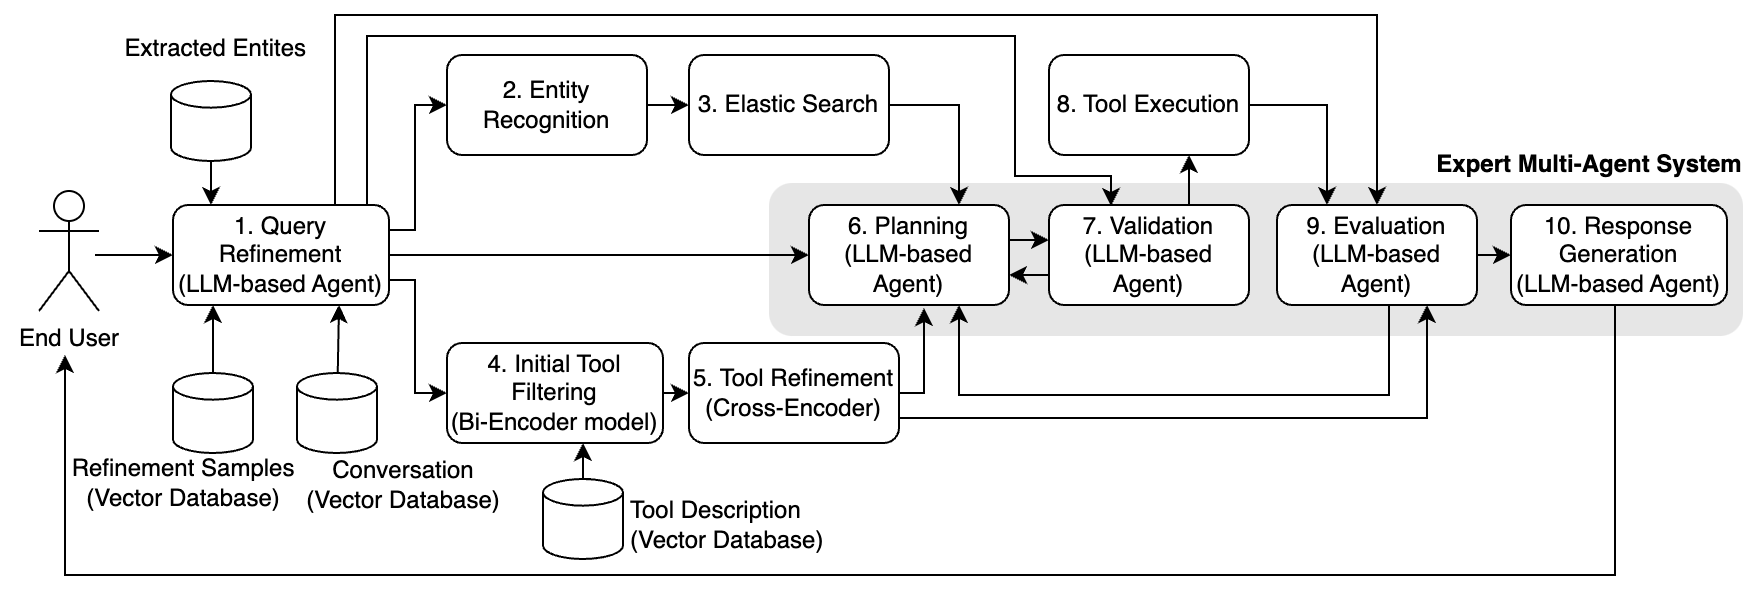
\includegraphics[width=\textwidth]{figures/architecture.png}
    \caption{Chatbot Architecture}
    \label{fig:architecture}
\end{figure}

To meet the diverse needs of users, the chatbot system integrates multiple tools (see Section~\ref{sec:chatbot_requirement}). These tools are used by feeding their descriptions and input parameters into the LLM prompt. Including all available tools in the prompt can reduce efficiency and increase costs due to the excessive information processing. To address this, we implement a filtering process for the tools using two models: \textit{Bi-Encoder} (Module 4) and \textit{Cross-Encoder} (Module 5) \cite{10.1145/3404835.3463076}. The \textit{Bi-Encoder} model first computes and stores  embeddings in a vector database for all tool descriptions. The embedding of user's query then is compared with every stored  embeddings to identify which tools are most likely to meet the current query’s needs. %This enables the Bi-Encoder to perform fast, efficient initial filtering, reducing the number of tools that require further processing.
Once the \textit{Bi-Encoder} selects potential tools, the \textit{Cross-Encoder} re-ranks them. Unlike the \textit{Bi-Encoder}, the \textit{Cross-Encoder} processes the input as pairs of the user’s query and tool descriptions. It outputs a similarity score ranging from 0 to 1, indicating the degree of relevance between the query and each tool description. The \textit{Cross-Encoder} excels at capturing the relationship between the query and tool descriptions, resulting in higher accuracy compared to the \textit{Bi-Encoder}. However, it is slower because it does not precompute and store embeddings for tool descriptions as the \textit{Bi-Encoder} does.

% Once the Bi-Encoder selects potential tools, the Cross-Encoder re-ranks them. 
% Cross-Encoder không tạo ra các embedding riêng lẻ cho từng câu như Bi-Encoder. Cross-Encoder nhận đầu vào là cặp câu hỏi và mô tả công cụ và trả về một giá trị đầu ra nằm trong khoảng từ 0 đến 1, biểu thị mức độ tương đồng của cặp câu này. Cross-Encoder có khả năng nắm bắt được ngữ cảnh đầy đủ và mối quan hệ giữa tool description và user's query cặp câu nên có độ chính xác cao hơn Bi-Encoder. Tuy nhiên Cross-Encoder chậm hơn do không thể lưu trữ sẵn phần nhúng của mô tả công cụ cần truy xuất như Bi-Encoder.

% Although the Cross-Encoder is slower as it processes both the query and tool descriptions simultaneously, it is more accurate due to its deeper understanding of the similarity between the query and the tools. This ensures that only the most suitable tools are chosen for use in the agent system.

Next, Modules 6, 7, 9, and 10 work together as a multi-agent system, with Modules 6 and 9 serving as the core agents. Module 6, the \textit{Planning}, is an LLM-based agent that takes three inputs: (1) the refined query, (2) the identified entities and their detailed information, and (3) the list of tools filtered by the \textit{Bi-Encoder} and \textit{Cross-Encoder}. The \textit{Planning} is responsible for devising a plan to use the tools, including the order of execution and the detailed input parameters for each tool. %This plan is then validated by Module 7, the \textit{Validation}, and if approved, passed to Module 8.
If the \textit{Planning} determines that the available tools are unsuitable for the query, it will not generate a plan. In such cases, Module 7, the \textit{Validation}, assesses the \textit{Planner}’s decision to prevent errors or hallucinations. If the plan is deemed viable, it is passed to Module 8 for execution.

Module 8, the \textit{Tool Execution}, implements the plan. Its results are then passed to Module 9, the \textit{Evaluation}, another LLM-based agent. The \textit{Evaluation} receives the tools, the refined query, and the execution results from the \textit{Planning} to assess whether the plan meets the user’s needs. If the plan is insufficient and can be improved using available tools, the \textit{Evaluation} develops additional plans based on prior ones to optimize the outcome, and the process loops back to the \textit{Planning}.

If the plan meets the requirements, the \textit{Evaluation} notifies Module 10, the \textit{Response Generation}, to compile and deliver the final response to the user. In cases where the plan is not fully satisfactory and no further tools can improve the result, the \textit{Evaluation} still notifies the \textit{Response Generation}. This module will then summarize what has been resolved and acknowledge the unresolved issues to the end user.

The following section details the \textit{Question Refinement, Entity Recognition, Tool Filtering, Planning, Validation, Evaluation}, and \textit{Response Generation} modules.

% Details of the Question Refiner, Entity Recognizer, Tool Filters (Bi-Encoder and Cross-Encoder), Planner, Plan Validator, Evaluator, and Response Generator modules will be discussed in the following section.

\begin{comment}
Kiến trúc của chatbot được mô tả trong hình 1. Khi người dùng gửi câu hỏi đến chatbot, module Question refiner sẽ tinh chỉnh câu hỏi sẽ được viết lại cho rõ ràng hơn bởi module 1. Module này là 1 dạng LLM-based agent. Để điều chỉnh câu hỏi, chúng tôi sử dụng lịch sử hội thoại của người dùng được lưu trữ dưới dạng vector nhúng và các thực thể được trích xuất từ lịch sử hội thoại đó, để đưa vào prompt cho LLM agent. Dựa trên những thông tin này, LLM agent sẽ tạo ra một câu hỏi rõ ràng, độc lập và dễ hiểu hơn, nghĩa là câu hỏi chứa đủ thông tin và ý định hiện tại của người dùng mà không cần tham chiếu lại lịch sử hội thoại.
 
Câu hỏi đã được tinh chỉnh sẽ được chuyển qua các module 2, 4, và 6. Đầu tiên, câu hỏi đi qua module 2, là một mô hình nhận diện thực thể nhỏ gọn chỉ bao gồm bộ mã hóa để trích xuất các đoạn văn bản có khả năng là thực thể và xác định loại thực thể tương ứng. Đoạn văn bản này có thể là tên chính xác của thực thể hoặc gần đúng trong trường hợp người dùng nhập sai chính tả (ví dụ: "Bitcon" thay vì "Bitcoin"). Kết quả từ module 2 sau đó được đưa vào module 3, sử dụng công nghệ Elastic Search để tìm kiếm chính xác các thực thể và thông tin đặc tả liên quan. Mục đích của module này là bổ sung kiến thức về các thực thể còn thiếu cho mô hình ngôn ngữ lớn (LLM), vì LLM chỉ có thể nhận diện và hiểu các thực thể có trong dữ liệu huấn luyện của nó, trong khi việc mở rộng kiến thức thông qua huấn luyện LLM là tốn kém.

Để đáp ứng nhu cầu đa dạng của người dùng, hệ thống chatbot cần tích hợp nhiều công cụ khác nhau. Các công cụ này được sử dụng bằng cách đưa mô tả và các tham số đầu vào vào prompt cho mô hình ngôn ngữ lớn (LLM). Việc đưa tất cả công cụ vào prompt có thể gây giảm hiệu suất và tăng chi phí do LLM phải xử lý quá nhiều thông tin dư thừa.
Để giải quyết vấn đề này, chúng tôi thực hiện lọc trước công cụ bằng hai model dạng Bi-Encoder (module 4) và Cross-Encoder (module 5) \cite{10.1145/3404835.3463076}. Bi-Encoder tính toán các phần nhúng (embeddings) độc lập cho cả mô tả công cụ và truy vấn của người dùng. Bằng cách này, Bi-Encoder có thể lưu trữ sẵn phần nhúng của mô tả công cụ, cho phép nhanh chóng so sánh các vector nhúng để xác định những công cụ nào có khả năng đáp ứng nhu cầu truy vấn hiện tại. Điều này giúp Bi-Encoder thực hiện bước lọc sơ bộ một cách nhanh chóng và hiệu quả, giảm thiểu số lượng công cụ cần xử lý sâu hơn.
 
Sau khi Bi-Encoder chọn ra các công cụ tiềm năng, Cross-Encoder sẽ xếp hạng lại các công cụ này dựa trên mức độ phù hợp và độ chính xác. Cross-Encoder hoạt động chậm hơn vì phải xử lý truy vấn và mô tả công cụ đồng thời, nhưng chính xác hơn do khả năng hiểu sâu sắc sự tương tác giữa truy vấn và công cụ. Điều này đảm bảo rằng chỉ những công cụ thực sự phù hợp mới được chọn để đưa vào hệ thống tác tử.
 
Tiếp theo, các module 6, 7, 8 và 9 kết hợp tạo thành một hệ thống đa tác tử, với các tác tử cốt lõi là smodule 6 và 8. Module số 6, Planner là một LLM-based Agent nhận 3 đầu vào là (1) câu hỏi đã tinh chỉnh, (2) các thực thể nhận biết trong câu hỏi và các trường thông tin chi tiết của mỗi thực thể, và (3) danh sách các công cụ được lọc bởi Bi-Encoder và Cross-Encoder. Module này cần lên kế hoạch sử dụng công cụ, bao gồm thứ tự sử dụng công cụ và tham số đầu vào chi tiết cho từng công cụ.
 
Module 7 Executer nhận và thực hiện kế hoạch thực thi các công cụ. Kết quả thực thi được chuyển đến module Evaluator (module 8), cũng là một LLM-based agent. Evaluator agent nhận đầu vào là các công cụ, câu hỏi đã tinh chỉnh, cùng với kết quả thực thi kế hoạch từ Planner Agent, để đánh giá xem kế hoạch có đáp ứng đầy đủ yêu cầu của người dùng hay không. Nếu kế hoạch chưa đạt yêu cầu và có khả năng được cải thiện bằng các công cụ hiện có, Evaluator sẽ tiếp tục phát triển các kế hoạch bổ sung dựa trên các kế hoạch trước đó để tối ưu hóa kết quả và luồng xử lý trở lại module Planner.

Nếu kế hoạch đáp ứng yêu cầu, Evaluator sẽ gửi tín hiệu đến Module Response generator (module 9) để tổng hợp và cung cấp câu trả lời hoàn chỉnh cho người dùng. Trong trường hợp kế hoạch không hoàn toàn thỏa mãn yêu cầu nhưng không còn công cụ nào có thể cải thiện câu trả lời, Evaluator vẫn gửi tín hiệu đến Module Response generator. Module này sẽ tổng hợp những gì đã được giải quyết và thừa nhận những vấn đề còn chưa được giải quyết với người dùng cuối.
\end{comment}

\section{AI Models for Architectural Modules}
\label{sec:ai_model}

\subsection{Question Refinement Agent}
\label{section:5.1}

In a question-answering system, accurately understanding user queries is crucial. However, users often phrase questions incompletely or refer to previous questions, which can lead to misunderstandings of their intent. For instance, consider the sequence: \textit{``(1) What are the top ranking tokens now? (2) What is the current price of the third one? (3) How about its deposit rate on Venus lending pool?''}. Only the first query is complete and clear; the subsequent queries lack necessary information and depend on context from previous questions. Expecting users to provide all required details in every individual query is unrealistic and unnatural.

% Trong hệ thống hỏi đáp, việc hiểu đúng câu hỏi là một yêu cầu bắt buộc. Tuy nhiên, người dùng thường diễn đạt câu hỏi không đầy đủ, hoặc có nhiều tham chiếu tới các lượt hội thoại trước đó, dẫn đến hệ thống không thể nắm bắt đúng ý định của người dùng. Ví dụ với chuỗi câu hỏi sau: 1. \textit{What are the top ranking tokens now?}. 2. \textit{What is the current price of the third one?}. 3. \textit{How about its deposit rate on Venus lending pool?}, chỉ câu truy vấn đầu tiên là đầy đủ và rõ ràng; các câu truy vấn tiếp theo thiếu thông tin cần thiết và phụ thuộc vào ngữ cảnh từ các câu trước. Việc đòi hỏi người dùng luôn cung cấp đúng và đủ toàn bộ các thông tin cần thiết trong mỗi câu truy vấn đơn lẻ là điều không thể và thiếu tự nhiên.

To address this issue, we rewrite queries into  clear, standalone questions based on conversational context \cite{10.1145/3459637.3482164}. This method enhances response accuracy by refining the query into a more explicit form and reduces computational costs by processing only the refined query rather than the entire conversation history.
% Để giải quyết vấn đề này, chúng tôi đề xuất phương pháp viết lại truy vấn thành câu hỏi độc lập và rõ ràng dựa trên ngữ cảnh hội thoại \cite{10.1145/3459637.3482164}. Phương pháp này giúp tăng độ chính xác phản hồi, do câu hỏi sau khi tinh chỉnh đã trở nên rõ ràng. Chi phí tính toán cũng được tối ưu, vì chúng tôi chỉ cần đưa vào câu hỏi đã tinh chỉnh thay cho việc phải đưa vào toàn bộ lịch sử hội thoại để giúp chatbot hiểu ngữ cảnh câu hỏi.

% \begin{figure}[h!]
%     \centering
%     \includesvg[width=1.0\textwidth]{figures/API chatbot-Refine Agent.drawio.svg}
%     \caption{Question refinement agent.}
%     \label{fig:Question refinement agent}
% \end{figure}

The question refinement process employs two vector databases. First, the conversation history between the user and the system is stored as ``Question-Answer'' pairs, which are then vectorized and stored in the \textit{Conversation Vector Database} using Qdrant\footnote{\url{https://qdrant.tech/}}. Additionally, examples with the format ``conversation history -- original query -- refined query'' are created and stored in the \textit{Refinement Sample Vector Database} to guide the LLM in refining queries more accurately.

% Quá trình tinh chỉnh câu hỏi sẽ sử dụng 2 cơ sở dữ liệu vector. Đầu tiên, lịch sử trò chuyện giữa người dùng và hệ thống được lưu trữ lại dưới dạng các cặp “Câu hỏi - Câu trả lời”, sau đó được vector hoá và lưu trữ lại trong CSDL vector Qdrant\footnote{\url{https://qdrant.tech/}}. Tiếp đến các bộ ví dụ với cấu trúc “lịch sử hội thoại - truy vấn hiện tại - truy vấn đã được tinh chỉnh” cũng được tạo và lưu trữ lại trong CSDL vector, giúp hướng dẫn LLM tinh chỉnh câu hỏi chính xác hơn.

The LLM agent for query refinement utilizes three types of input data. (1) First, it identifies relevant segments of the conversation history by vectorizing the user's query and matching it with the \textit{Conversation History Vector Database}. This approach avoids processing all previous interactions. (2) It selects query refinement examples that are contextually relevant from the \textit{Refinement Sample Vector Database}. (3) It incorporates blockchain entities extracted from prior queries. These three inputs are combined in the prompts, allowing the LLM to refine queries effectively by leveraging its reasoning and language understanding capabilities.

% The LLM agent responsible for refining queries relies on three types of input data: (1) Relevant parts of the conversation history are identified so that we do not need to process every previous interaction. This is done by vectorizing user's query and match it with the Conversation History Vector Database. (2) Query refinement example gần với ngữ cảnh hội thoại are selected from the Refinement Sample Vector Database với cơ chế tương tự. Hai đầu vào này cùng với (3) các blockchain entities extracted from prior queries được đưa vào trong LLM promts để tận dụng khả năng suy luận và hiểu ngôn ngữ của LLm để perform the query refinement effectively.

% LLM tinh chỉnh câu hỏi cần 3 dữ liệu đầu vào. (1) Câu hỏi của người dùng được vector hóa để so khớp với CSDL vector lịch sử hội thoại, giúp tìm ra những phần lịch sử hội thoại liên quan tới câu hỏi, thay vì sử dụng toàn bộ các cuộc trò chuyện trước đó. (2) Ví dụ về tinh chỉnh truy vấn: Các ví dụ về nhiệm vụ tinh chỉnh truy vấn được trích chọn từ cơ sở dữ liệu ví dụ, với yêu cầu phải gần với ngữ cảnh hội thoại hiện tại. Những ví dụ này bao gồm cấu trúc “lịch sử hội thoại - truy vấn hiện tại - truy vấn đã được tinh chỉnh” và đóng vai trò hướng dẫn LLM cho việc tinh chỉnh câu hỏi. (3) Các thực thể Blockchain đã được nhận diện ở các truy vấn trước sẽ được lấy ra. 3 dữ liệu đầu vào này sẽ được cung cấp cho LLM agent thực hiện tinh chỉnh câu hỏi. 

%Các mô hình nhúng dạng Bi-encoder \cite{10.1145/3404835.3463076} giúp mã hóa văn bản và các thông tin liên quan thành các vector riêng biệt, sau đó so sánh độ tương đồng giữa chúng một cách nhanh chóng và hiệu quả, tiết kiệm tài nguyên tính toán. Trong các hệ thống hỏi đáp, một số mô hình bi-encoder nổi tiếng bao gồm DPR[], Contriever[], BGE [], LLM-Embedder \cite{DBLP:journals/corr/abs-2310-07554}. Trong bài toán của chúng tôi, để trích xuất được lịch sử hội thoại liên quan và ví dụ tương đồng, chúng tôi chọn LLM-Embedder làm mô hình nhúng để vector hoá và so sánh độ tương đồng giữa các thành phần sau: (i) truy vấn của người dùng, (ii) lịch sử hội thoại, (iii) ví dụ về việc tinh chỉnh. Lý do chúng tôi chọn mô hình LLM-embedder là vì nó rất linh hoạt với khả năng xử lý nhiều nhiệm vụ khác nhau như knowledge retrieval, memory augmentation, in-context learning through example retrieval, và tool selection. Thay vì phải sử dụng mô hình nhúng riêng cho từng nhiệm vụ, LLM- Embedder hợp nhất các chức năng truy xuất khác nhau thành một mô hình duy nhất. Điều này không những giúp tiết kiệm tài nguyên mà hiệu suất của mô hình cũng được cải thiện do mô hình học hỏi được từ nhiều ngữ cảnh và nhiệm vụ khác nhau và trở nên toàn diện và hiệu quả hơn.

% Triển khai các ý cho việc giới thiệu LLM-Embedder trong bài toán
% - Tóm gọn lại LLM Embedder là mô hình nhúng, làm rõ để tránh người đọc hiểu nhầm
% - Nói rõ đây là mô hình đa tác vụ và mình sử dụng 3 tác vụ trong số đó
% - Nói về cách xử lý fine tune cho các vị trí khác nhau

%Để làm việc với các biểu diễn vector như đã đề cập ở trên, chúng ta cần một mô hình nhúng dạng bi-encoder \cite{10.1145/3404835.3463076} để mã hoá văn bản thành các biểu diễn trong không gian vector. Trong bài toán của chúng tôi, chúng tôi cần các biểu diễn vector cho 3 tác vụ sau memory augmentation (so khớp câu hỏi người dùng với lịch sử hội thoại - (1) trong đoạn trên), example retrieval (ví dụ về tinh chỉnh truy vấn - (2) trong đoạn trên), tool selection (Phần lọc tool 5.3). Thay vì mỗi tác vụ cần phải sử dụng một model nhúng độc lập, chúng tinh chỉnh và sử dụng mô hình nhúng LLM-Embedder (109M parameters) \cite{DBLP:journals/corr/abs-2310-07554} vì mô hình này rất linh hoạt với khả năng xử lý nhiều nhiệm vụ khác nhau như knowledge retrieval, memory augmentation, in-context learning through example retrieval, và tool selection bằng kỹ thuật fine-tuning dựa trên hướng dẫn (Instruction-based Fine-Tuning). Cụ thể, mỗi tác vụ sẽ được gán với một hướng dẫn cụ thể, nhằm đảm bảo rằng các embedding được điều chỉnh phù hợp cho từng tác vụ khác nhau. Mỗi hướng dẫn (instruction) sẽ có 1 cặp "Query", "Key", lần lượt là hướng dẫn dành cho truy vấn của người dùng và hướng dẫn dành cho thông tin truy xuất từ cơ sở dữ liệu vector. Cụ thể, với tác vụ example retrieval, đầu vào của LLM-Embdder lần lượt là:
We employ the LLM-Embedder model \cite{DBLP:journals/corr/abs-2310-07554}, with 109 million parameters, to encode text into vector space. This bi-encoder model is versatile, capable of handling tasks such as \textit{knowledge retrieval}, \textit{memory augmentation}, \textit{in-context learning through example retrieval}, and \textit{tool selection} by leveraging instruction-based fine-tuning technique.

These tasks are highly relevant to our chatbot system. \textit{Memory augmentation} retrieves relevant conversation history, used in the question refinement agent, while \textit{in-context learning} allows the retrieval of similar examples for query refinement; \textit{tool selection} is applied to identify the appropriate tools to answer user queries (see Section~\ref{sec:tool_filtering}). Due to the challenges of data generation and the strong performance of the base model, we did not fine-tune the LLM-Embedder for the first two tasks. Fine-tuning was applied solely for the tool selection task, details of which are presented in Section~\ref{sec:tool_filtering}.

% Chúng tôi sử dụng mô hình nhúng LLM-Embedder \cite{DBLP:journals/corr/abs-2310-07554} với 109 triệu tham số để mã hóa văn bản vào không gian vector. Đây là một mô hình bi-encoder linh hoạt, có khả năng xử lý nhiều tác vụ khác nhau như knowledge retrieval, memory augmentation, in-context learning through example retrieval, và tool selection, thông qua kỹ thuật fine-tuning dựa trên hướng dẫn (Instruction-based Fine-Tuning). Các tác vụ này rất phù hợp với bài toán chatbot của chúng tôi. Memory augmentation giúp truy xuất lịch sử hội thoại liên quan, được dùng trong Agent tinh chỉnh câu hỏi; in-context learning through example retrieval cho phép tìm ví dụ tương đồng cho tinh chỉnh truy vấn; tool selection được dùng để lọc ra các công cụ cần sử dụng để trả lời câu hỏi cho người dùng (see Section~\ref{sec:tool_filtering}). Với 2 tác vụ đầu, do khó khăn trong việc tạo dữ liệu và qua thực nghiệm mô hình gốc đã đạt hiệu năng cao rồi nên chúng tôi không thực hiện fine tune mô hình LLM-embedder. Chúng tôi chỉ fine tune cho mô hình LLM-embedder dùng trong tác vụ tool selection. Chi tiết trình bày trong Section~\ref{sec:tool_filtering}.

Each task is assigned a specific instruction, consisting of a \textbf{Query} and a \textbf{Key} pair, to guide the LLM-Embedder in adjusting vector representations according to the task requirements \cite{asai-etal-2023-task,DBLP:journals/corr/abs-2310-07554,INSTRUCTOR}. The \textbf{Query} instruction is applied to user queries, and the \textbf{Key} instruction is used for embedding information stored in the vector database. For example, in the task of finding relevant examples for query refinement, the \textbf{Query} instruction is: ``\textit{Convert the following dialogue into vector to find useful examples: User Question}'' while the \textbf{Key} instruction is: ``\textit{Convert this example into vector for retrieval: Example}''.


% Để xử lý nhiều tác vụ, mỗi tác vụ được gán với một hướng dẫn cụ thể (instruction) bao gồm một cặp "Query" và "Key" để mô hình LLM-embedder thay đổi biểu diễn vector nhúng sao cho phù hợp với yêu cầu riêng của từng nhiệm vụ \cite{asai-etal-2023-task,DBLP:journals/corr/abs-2310-07554}. Trong đó, hướng dẫn "Query" áp dụng cho truy vấn của người dùng và "Key" áp dụng cho các thông tin cần được nhúng để lưu trữ trong cơ sở dữ liệu vector. Ví dụ với nhiệm vụ tìm ví dụ tinh chỉnh câu hỏi tương đồng, hướng dẫn Query là: ``\textit{Convert the following dialogue into vector to find useful examples: User Question}'' và hướng dẫn Key là: ``\textit{Convert this example into vector for retrieval: Example}''

%Mỗi tác vụ được gán với một hướng dẫn cụ thể (instruction) dưới dạng cặp "Query" và "Key," để điều chỉnh embedding sao cho phù hợp với từng nhiệm vụ \cite{asai-etal-2023-task, DBLP:journals/corr/abs-2310-07554}. Cụ thể, việc thêm các hướng dẫn này vào trước văn bản cần tính toán vector sẽ thay đổi biểu diễn vector để phù hợp với yêu cầu của từng tác vụ. Mỗi hướng dẫn (instruction) sẽ có 1 cặp "Query", "Key", lần lượt là hướng dẫn dành cho truy vấn của người dùng và hướng dẫn dành cho thông tin truy xuất từ cơ sở dữ liệu vector. Ví dụ, với tác vụ tìm ví dụ tương đồng cho tinh chỉnh truy vấn (in-context learning through example retrieval), các hướng dẫn đầu vào cho LLM-Embedder là:

% \begin{itemize}
% \item \textbf{Query:} \textit{"Convert the following dialogue into vector to find useful examples:} $+$ \textbf{User Question}
% \item \textbf{Key:} \textit{"Convert this example into vector for retrieval:"} $+$ \textbf{Example}
% \end{itemize}

%Như vậy, bằng cách thêm instruction đặc biệt bao gồm \textit{"Query"} và \textit{"Key"} trước khi tiến hành vector hoá văn bản, biểu diễn vector đầu ra của LLM-Embdder sẽ được điều chỉnh cho phù hợp với tác vụ đó.

% Nhờ việc thêm các hướng dẫn "Query" và "Key" trước khi vector hóa văn bản, LLM-Embedder điều chỉnh biểu diễn vector để phù hợp với tác vụ cụ thể, tối ưu hóa hiệu suất cho từng nhiệm vụ.

% Để trích xuất được lịch sử hội thoại liên quan và ví dụ tương đồng, chúng tôi tiến hành so khớp ngữ nghĩa bằng cách vector hóa văn bản,  sử dụng mô hình nhúng LLM-Embedder \cite{DBLP:journals/corr/abs-2310-07554}, một dạng mô hình bi-encoder, không phải LLM, mà được thiết kế để tăng cường khả năng của LLM thông qua truy xuất dữ liệu \cite{10.1145/3404835.3463076}. Bi-encoder giúp mã hóa văn bản và các thông tin liên quan thành các vector riêng biệt, sau đó so sánh độ tương đồng giữa chúng một cách nhanh chóng và hiệu quả, tiết kiệm tài nguyên tính toán. Mô hình LLM-embedder rất linh hoạt với khả năng xử lý nhiều nhiệm vụ khác nhau như knowledge retrieval, memory augmentation, in-context learning through example retrieval, và tool selection. Thay vì phải sử dụng mô hình nhúng riêng cho từng nhiệm vụ, LLM- Embedder hợp nhất các chức năng truy xuất khác nhau thành một mô hình duy nhất. Điều này không những giúp tiết kiệm tài nguyên mà hiệu suất của mô hình cũng được cải thiện do mô hình học hỏi được từ nhiều ngữ cảnh và nhiệm vụ khác nhau và trở nên toàn diện và hiệu quả hơn.

% LLM-Embedder được thiết kế để tăng cường khả năng của LLM thông qua việc truy xuất dữ liệu bên ngoài. Mô hình này được huấn luyện trên dữ liệu đa tác vụ, mỗi tác vụ có một hướng dẫn riêng (instruction) \cite{asai-etal-2023-task}. Nhờ vào module attention trong kiến trúc transformer \cite{10.5555/3295222.3295349}, LLM-Embedder có thể tính toán phần nhúng hợp lý cho từng tác vụ dựa vào instruction cụ thể. Những instruction này giúp mô hình hiểu rõ yêu cầu và ngữ cảnh của từng nhiệm vụ, từ đó tạo ra các biểu diễn vector phù hợp.


\subsection{Entity Recognition with GLiNER and Elastic Search}

Accurate recognition of blockchain entities (e.g., tokens, projects, chains) is essential for our chatbot architecture, as it ensures correct understanding of user queries and appropriate tool selection. However, entity recognition encounters several challenges: (i) the extensive variety of entities, (ii) the continual introduction of new entities, (iii) the interchangeability of names and symbols, and (iv) the absence of standardized naming conventions, leading to potential name overlaps. For example, the token ``Bitcoin'' has the symbol ``BTC'', while ``blackrocktradingcurrency" also uses ``BTC.'' Thus, queries like ``What is the current BTC price?'' necessitate accurate differentiation between these entities.

% Việc nhận dạng đúng thực thể blockchain (e.g, token, project, chain) đóng vai trò quan trọng trong kiến trúc của chatbot. Nhận dạng thực thể gặp phải nhiều thách thức: (i) Số lượng thực thể rất lớn, (ii) Các thực thể mới được sinh ra liên tục, (iii) Người dùng có thể sử dụng cả tên và ký hiệu thay thế lẫn cho nhau khi nhắc tới một thực thể nào đó, (iv) Không có quy chuẩn hoặc dấu hiệu nhận biết gì về tên thực thể, thực thể này có thể có tên giống với thực thể khác.
% Nhìn chung, LLMs vẫn có khả năng nhận dạng được các thực thể trong câu truy vấn của người dùng nhưng chúng không đạt được hiệu quả cao trong miền Blockchain do các khó khăn đã nêu ở trên. Ngoài ra, việc truy xuất công cụ đòi hỏi một số trường thông tin đặc biệt của các thực thể, và các thông tin này thường sẽ nằm ngoài kiến thức và khả năng suy luận của LLMs.
% Ví dụ, mỗi token đều có tên (name) và ký hiệu (symbol). Token "Bitcoin" có ký hiệu là "btc" và tên là "Bitcoin", trong khi như token "blackrocktradingcurrency" cũng có ký hiệu "btc". Vì người dùng thường hỏi dạng "What is the current BTC price?", chúng ta phải hiểu BTC có thể là bitcoin và cũng có thể là blackrocktradingcurrency.


Our approach to entity recognition involves two steps: extracting potential entity strings from user queries using the GLiNER model \cite{zaratiana2023glinergeneralistmodelnamed}, and employing Elastic Search with BM25, Fuzzy Search, Prefix, and Wildcard algorithms to find the closest matching entity from our continuously updated and expanded entity database.
% Chúng tôi thực hiện nhận dạng thực thể theo 2 bước: (1) Trích xuất xâu có khả năng là thực thể từ truy vấn của người dùng, sử dụng mô hình GLINER \cite{zaratiana2023glinergeneralistmodelnamed} và (2) sử dụng công nghệ tìm kiếm ElasticSearch với các giải thuật BM25, Fuzzy Search, Prefix, Wildcard để tìm kiếm thực thể gần nhất với xâu đó, dựa trên cơ sở dữ liệu thực thể chuẩn bị từ trước.
This method offers several advantages: (i) GLiNER, a lightweight language model with approximately 400 million parameters, ensures high efficiency in entity recognition, and (ii) the entity database is continuously updated independently of GLiNER, enabling recognition of future entities without retraining and effectively handling misspelled entities.

% Cách làm này đem đến nhiều lợi ích.  (i) GLiNER là một mô hình ngôn ngữ nhỏ và nhẹ với khoảng 400 triệu tham số, đem lại hiệu năng cao về việc nhận diện xâu thực thể. (ii) Kho dữ liệu về thực thể được cập nhật liên tục, độc lập với mô hình GLiNER. (iii) Cơ chế 2 bước này giúp nhận dạng được cả các thực thể xuất hiện trong tương lai và các thực thể bị người dùng viết sai chính tả.

GLiNER \cite{zaratiana2023glinergeneralistmodelnamed} is designed for Named Entity Recognition (NER) and presents notable improvements over traditional NER systems and LLMs. Unlike traditional NER models restricted to fixed entity types, GLiNER can recognize various entity types using natural language prompts. This flexibility allows it to adapt to different domains without extensive retraining. To enhance the accuracy of entity recognition, we fine-tuned GLiNER.



% GLiNER \cite{zaratiana2023glinergeneralistmodelnamed}, là một mô hình dành cho tác vụ nhận dạng thực thể (NER), mang lại nhiều lợi thế và cải tiến kỹ thuật so với các hệ thống NER truyền thống cũng như các mô hình ngôn ngữ lớn (LLMs). Một trong những điểm mạnh nổi bật của GLiNER là tính linh hoạt trong việc nhận diện một loạt các loại thực thể. Không giống như các mô hình NER truyền thống bị giới hạn trong một tập hợp các loại thực thể cố định, GLiNER có thể trích xuất bất kỳ loại thực thể nào bằng cách sử dụng hướng dẫn ngôn ngữ tự nhiên. Khả năng nhận diện thực thể mở này làm cho mô hình có thể thích ứng với nhiều lĩnh vực khác nhau mà không cần phải huấn luyện lại rộng rãi để xử lý các loại thực thể mới. Để nâng cao hiệu quả và độ chính xác của module nhận dạng thực thể, chúng tôi đã tinh chỉnh mô hình GLiNER.

\begin{comment}

\begin{figure}[h!]
    \centering
    \includesvg[width=1.0\textwidth]{figures/API chatbot-NER.drawio.svg}
    \caption{Entitiy regconition and retrieval.}
    \label{fig:Entitiy regconition and retrieval}
\end{figure}

Hình \ref{fig:Entitiy regconition and retrieval} mô tả chi tiết quy trình nhận diện thực thể của hệ thống, bao gồm các bước sau:
(i) Trích xuất thực thể bằng GLINER: Sử dụng GLINER để trích xuất các xâu thực thể từ câu truy vấn đã được tinh chỉnh từ bước trước (\ref{section:5.1}). GLINER tận dụng các mô hình BiLM như BERT hoặc deBERTa để mã hóa văn bản và tạo ra các biểu diễn ngữ cảnh hóa cho các thực thể.
(ii) Elasticsearch cùng với MongoDB: các xâu thực thể sau khi được trích xuất từ truy vấn sẽ được đưa vào tìm kiếm bên trong Elasticsearch với các truy vấn và thuật toán khác nhau, nhằm tìm kiếm, trích xuất tất cả các thực thể tiềm năng so với truy vấn của người dùng.
(iii) Cung cấp dữ liệu về thực thể cho LLM: các thực thể sau khi được trích xuất cùng với các thông tin của chúng sẽ được đưa vào prompt cho LLM như là ngữ cảnh, từ đó giúp LLM có thể xử lý các bước tiếp theo chính xác và hiệu quả hơn.


Về mặt kỹ thuật, GLiNER tận dụng các mô hình ngôn ngữ song hướng (BiLM) như BERT và DeBERTa để trích xuất thực thể. Một khía cạnh cốt lõi của cơ chế GLiNER là ghép nối các biểu diễn của loại thực thể với các đoạn văn bản trong một không gian tiềm ẩn chung. Thay vì coi NER là một tác vụ sinh văn bản, GLiNER tập trung vào việc xác định sự tương thích ngữ nghĩa giữa các loại thực thể và các đoạn văn bản, dẫn đến độ chính xác cao hơn khi trích xuất thực thể. Hai thành phần quan trọng trong kiến trúc của GLiNER là Bộ mã hoá văn bản được huấn luyện sẵn (Pre-trained Textual Encoder) và module biểu diễn đoạn (Span Representation Module). Sau đây, chúng tôi sẽ nêu lại những điểm nổi bật của 2 thành phần này để từ đó có thể đưa ra được phương thức tinh chỉnh mô hình cho bài toán của chúng tôi.

Pre-trained Textual Encoder chịu trách nhiệm tạo ra các biểu diễn ngữ cảnh hóa của các token trong văn bản đầu vào, thông qua các mô hình ngôn ngữ song hướng (BiLM) như BERT hoặc DeBERTa. Trong GLiNER, định dạng đầu vào bao gồm hai phần: các loại thực thể cần được nhận diện và câu hoặc văn bản đầu vào. Các loại thực thể được biểu diễn bằng cách sử dụng các token đặc biệt được ký hiệu là [ENT], được chèn trước mỗi loại thực thể trong chuỗi đầu vào. Token [SEP] được sử dụng như một dấu phân cách giữa các loại thực thể và văn bản đầu vào. Chuỗi hợp nhất này sau đó được đưa vào bộ mã hóa đã được huấn luyện sẵn, bộ mã hóa này xử lý toàn bộ chuỗi để tạo ra các biểu diễn cấp token, nắm bắt các tương tác giữa tất cả các token. Kết quả đầu ra của bộ mã hoá là một loạt các biểu diễn vector cho mỗi token trong chuỗi đầu vào. Cụ thể, $p = \{ p_i \}_{i=0}^{M-1}$
là biểu diễn cho mỗi token kiểu thực thể, $h = \{ h_i \}_{i=0}^{N-1}$ là biểu diễn cho mỗi từ trong văn bản đầu vào. Trong đó, M là số lượng token kiểu thực thể, N là số lượng token từ. Các biểu diễn từ này là cơ sở để tính toán khoảng và khớp kiểu thực thể.

Span Representation Module tính toán biểu diễn đoạn (span) từ các biểu diễn token do bộ mã hóa văn bản tiền huấn luyện cung cấp. Nó giúp mô hình xác định những khoảng văn bản nào tương ứng với các thực thể bằng cách khớp chúng với các kiểu thực thể. Với một đoạn bắt đầu tại vị trí \textit{i} và kết thúc tại vị trí \textit{j}, biểu diễn đoạn $S_{ij}$ được tính toán theo công thức $S_{ij} = FFN(h_i \oplus h_j)$, với ý nghĩa là khoảng bắt đầu tại vị trí \textit{i} và kết thúc tại vị trí \textit{j} được biểu diễn bằng cách nối ($\oplus$) các token của từ bắt đầu và từ kết thúc, sau đó đưa qua mạng Neural FeedForward (\textit{FFN}) để tính toán biểu diễn đoạn $S_{ij}$
\end{comment}


Training data was generated using GPT-4 Turbo through the following process: (i) generating text segments containing blockchain-related entities and topics, annotated with XML syntax to mark entity positions, (ii) diversifying the entities and topics to enrich the data, and (iii) augmenting the data by altering entity names within XML tags, creating multiple variants with the same grammatical structure to enhance the model's ability to recognize entities based on sentence patterns rather than specific names.

% Để tạo dữ liệu huấn luyện với 1 số lượng lớn, không bị tác động bởi các yếu tố con người, chúng tôi sử dụng GPT-4 Turbo với quy trình: (i) Sinh các đoạn văn bản chứa các thực thể và chủ đề liên quan đến blockchain, đánh dấu vị trí của các thực thể thông qua cú pháp XML, (ii) Kết hợp nhiều thực thể và chủ đề khác nhau trong các văn bản để làm đa dạng và phong phú dữ liệu, (iii) Tăng cường dữ liệu bằng cách thay đổi tên các thực thể cùng loại trong các thẻ XML, tạo ra nhiều biến thể dữ liệu với cùng cấu trúc, từ đó tăng cường khả năng nhận dạng thực thể của mô hình dựa trên cả cấu trúc câu.

% Thông qua quy trình trên, chúng tôi mong muốn tinh chỉnh mô hình GLiNER giúp cho mô hình có thể nhận dạng được cả các thực thể mới trong tương lai, không chỉ bị giới hạn trong kiến thức của GPT-4 Turbo, cũng như giúp mô hình có thể nhận dạng được các thực thể bị viết sai trong câu truy vấn của người dùng.

% Ví dụ về dữ liệu tạo bởi GPT 4-Turbo: \textit{"In the rapidly evolving world of finance, <token cryptocurrency>Ethereum</token cryptocurrency> has emerged as a significant player. Investors are increasingly interested in how these digital assets interact with <lending pool>Compound Finance</lending pool>, allowing them to leverage their holdings for additional gains. Meanwhile, blockchain enthusiasts are keenly watching developments on the <chain>Binance Smart Chain</chain> due to its low transaction fees and fast processing times."}

% Nhằm đảm bảo rằng dữ liệu được chuẩn bị đúng cách để sử dụng trong việc tinh chỉnh mô hình GLINER, chúng tôi thực hiện quá trình tiền xử lý dữ liệu như sau (i) Loại bỏ các mẫu dữ liệu sai định dạng, (ii) Văn bản sau khi loại bỏ thẻ XML được chia thành các token, (iii) Nhận diện và gán nhãn thực thể dựa trên các thẻ XML trong văn bản ban đầu. Ví dụ về dữ liệu sau khi tiền xử lý: Văn bản được sinh ra: \textit{"In the rapidly evolving world of finance, Ethereum has emerged as a significant player. Investors are increasingly interested in how these digital assets interact with Compound Finance, allowing them to leverage their holdings for additional gains."}, nhãn thực thể: {(7, 7, "token cryptocurrency"), (12, 13, "lending pool"), (16, 18, "chain")}.

The resulting training dataset comprises 10,000 samples of text containing blockchain-related entities. The core model, deBERTa-v3, is a bidirectional language model with high performance in NER tasks. GLiNER’s non-pretrained layers have a width of 768 and a dropout rate of 0.4. Training utilized the AdamW optimizer, with a base learning rate of 1e-5 for the backbone transformer and 5e-5 for non-pretrained layers. Negative Entity Sampling with a ratio of 0.5 was employed to help the model distinguish between genuine entities and non-entities.
% Kết quả thu được tập dữ liệu huấn luyện bao gồm 10,000 mẫu, mỗi mẫu chứa các đoạn văn bản với các thực thể thuộc lĩnh vực blockchain. Thành phần chính của mô hình là deBERTa-v3, một mô hình ngôn ngữ hai chiều (BiLM) nổi bật với hiệu suất cao trong các tác vụ nhận dạng thực thể. Các lớp không được tiền huấn luyện của GLINER có chiều rộng là 768 và tỷ lệ dropout là 0.4.
% Quá trình huấn luyện sử dụng AdamW optimizer, với learning rate cơ bản 1e-5 cho backbone transformer và 5e-5 cho các lớp không được tiền huấn luyện. Kỹ thuật Negative Entity Sampling với tỉ lệ 0.5 giúp mô hình học cách phân biệt thực thể thực sự và từ không phải thực thể.



\subsection{Tool Filtering with Bi-Encoder and Cross-Encoder Models}
\label{sec:tool_filtering}
Incorporating tools is essential for bridging LLMs with real-time data. For example, a tool that accepts a token name and returns its price allows the LLM to answer questions like \textit{``What is the current price of Bitcoin?''}. A chatbot equipped with multiple tools can address diverse user requests. However, integrating too many tool descriptions into the LLM increases context length and complexity, leading to the \textbf{lost in the middle} issue \cite{liu-etal-2024-lost}, where the LLM tends to forget critical information midway through, making it difficult to accurately select the right tool.


% Công cụ là thành phần quan trọng trong việc kết nối mô hình ngôn ngữ lớn (LLM) với thế giới theo thời gian thực. Một công cụ nhận đầu vào là tên token và trả về giá của nó có thể hỗ trợ LLM trả lời các câu hỏi như \textit{“What is the current price of Bitcoin?”} Chatbot được tích hợp nhiều công cụ khác nhau sẽ đáp ứng các yêu cầu đa dạng của người dùng. Tuy nhiên, việc đưa quá nhiều công cụ và mô tả của chúng vào LLM agent làm tăng độ dài và sự phức tạp của ngữ cảnh, dẫn đến hiện tượng "lost in the middle" \cite{liu-etal-2024-lost}, khiến LLM có xu hướng quên thông tin ở giữa và không thể hoàn thành nhiệm vụ chọn chính xác công cụ cũng như đầu vào của chúng.


% \begin{figure}[h!]
%     \centering
%     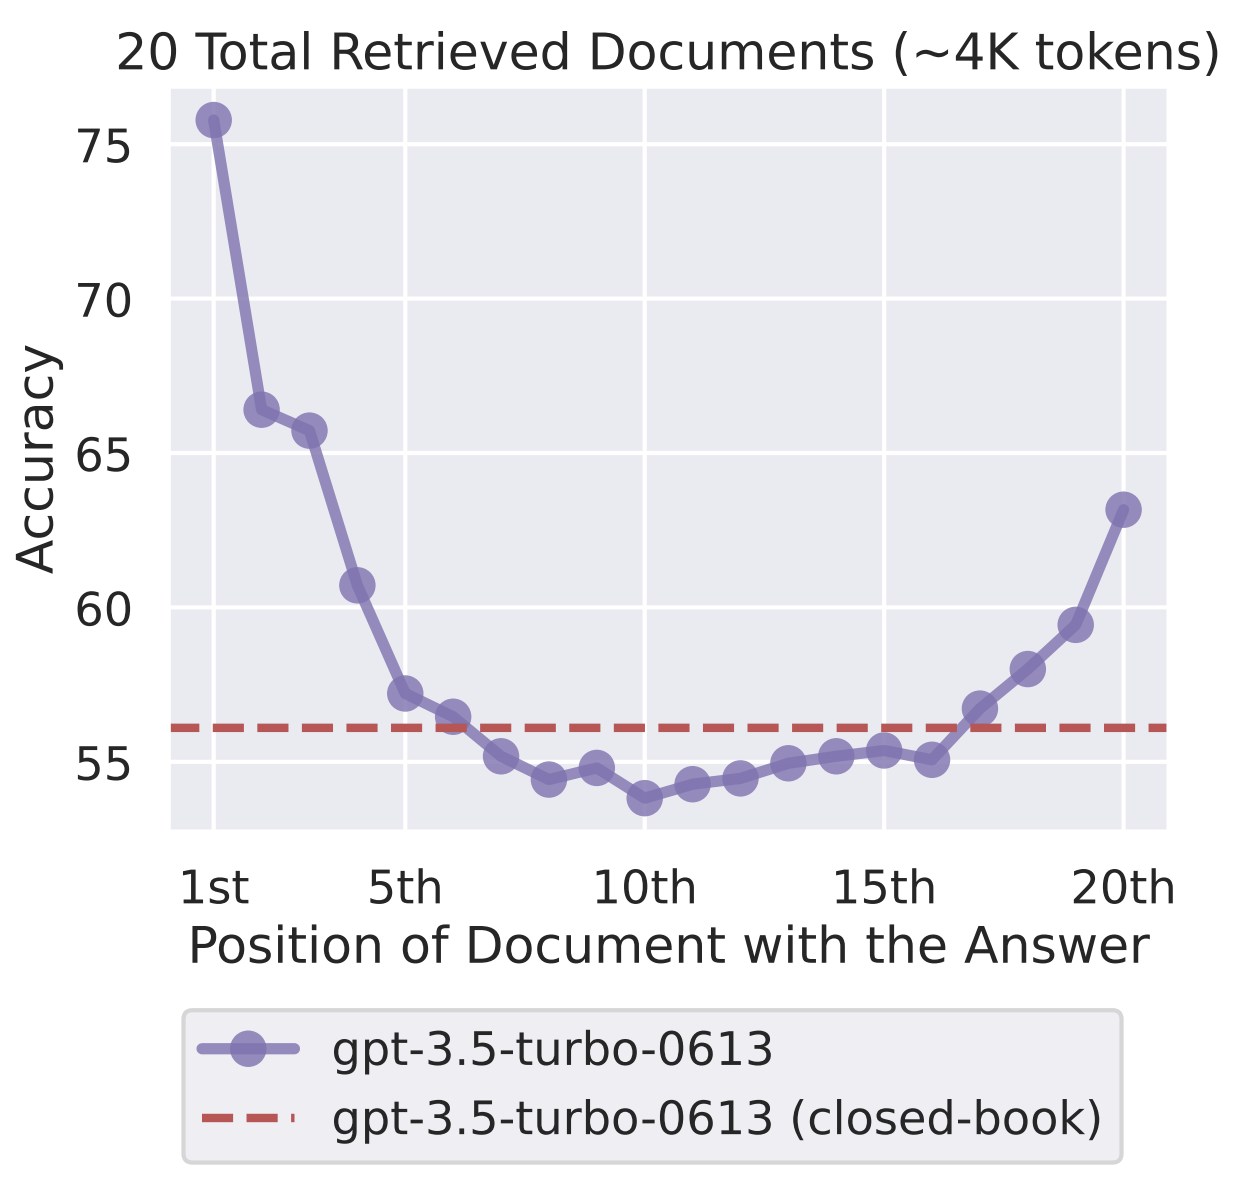
\includegraphics[width=0.5\textwidth]{figures/lost_in_middle.png}
%     \caption{Language model tends to "forget" the middle information}
%     \label{fig:Language model tends to "forget" the middle information}
% \end{figure}

% Trong hình \ref{fig:Language model tends to "forget" the middle information}, đường nét liền “open-book” đại diện cho mức độ chính xác của LLM khi sử dụng các văn bản bên để trả lời, còn đường nét đứt “closed-book” đại diện cho mức độ chính xác của LLM khi trả lời bằng chính kiến thức đã được huấn luyện. Biểu đồ cho thấy độ chính xác của mô hình GPT-3.5 Turbo giảm mạnh khi thông tin cần truy vấn nằm ở giữa ngữ cảnh (từ vị trí văn bản thứ 5 đến 15). Điều này cho thấy LLM thường quên thông tin quan trọng ở giữa đoạn văn bản, làm giảm khả năng xử lý thông tin. Việc kiểm soát độ dài ngữ cảnh là rất quan trọng để duy trì hiệu quả của LLM, đặc biệt là trong các tác vụ yêu cầu giữ lại và sử dụng toàn bộ thông tin để đưa ra câu trả lời chính xác như việc chọn công cụ và đầu vào của chúng. Lý do là vì chúng ta phải đưa thông tin cho LLM về toàn bộ các công cụ, kèm theo mô tả về cách sử dụng và các đầu vào của công cụ

To address this, irrelevant tools must be filtered out before passing their description to the LLM. The tool filtering process involves two stages. First, the refined query (see Section~\ref{section:5.1}) is vectorized using LLM Embedder \cite{DBLP:journals/corr/abs-2310-07554}, a Bi-Encoder model, and matched with pre-embedded tool descriptions stored in a vector database. This initial step filters out the most relevant tools. Next, these candidate tools are re-ranked by the BGE Rerank\footnote{\url{https://huggingface.co/BAAI/bge-reranker-base}}, a Cross-Encoder model, which assigns scores to find the tools most appropriate for the query. This two-stage filtering process improves scalability, reduces computational cost, and enhances accuracy \cite{10.1145/3404835.3463076}.

% Do đó, chúng ta cần loại bỏ bớt các công cụ không phù hợp trước khi chuyển cho LLM. Công cụ được lọc theo 2 bước. Trước tiên, câu truy vấn đã được tinh chỉnh (see Section~\ref{section:5.1}) được vector hóa thông qua LLM Embedder, một mô hình Bi-Encoder, rồi so khớp với các mô tả công cụ đã được nhúng và lưu trữ trong CSDL vector để lọc ra các công cụ tiềm năng nhất. Sau đó, các công cụ ứng viên này sẽ được tính điểm và xếp hạng bằng mô hình BGE rerank \cite{huggingface_bge_reranker}, một mô hình Cross-Encoder, nhằm tìm ra những công cụ phù hợp nhất với truy vấn của người dùng. Việc kết hợp lọc hai bước giúp tăng khả năng mở rộng, tối ưu chi phí cũng như độ chính xác \cite{10.1145/3404835.3463076}.


% \begin{figure}[h!]
%     \centering
%     \includesvg[width=1.0\textwidth]{figures/API chatbot-Tool selection.drawio.svg}
%     \caption{Tool selection.}
%     \label{fig:Tool selection.}
% \end{figure}

\begin{comment}    
LLM-Embedder có khả năng điều chỉnh vector nhúng dựa trên các hướng dẫn cụ thể cho từng nhiệm vụ như đã đề cập ở phần cuối của \ref{section:5.1}. Các hướng dẫn này ảnh hưởng đến các trạng thái ẩn cuối cùng của tất cả các token thông qua self-attention module. Cụ thể, với tác vụ truy xuất công cụ (tool selection), hướng dẫn sẽ bao gồm:

\begin{itemize}
\item \textbf{Query:} \textit{"Transform this user request for fetching helpful tool descriptions:"} $+$ \textbf{User Question}
\item \textbf{Key:} \textit{"Transform this tool description for retrieval:"}  $+$ \textbf{Tool Description}
\end{itemize}

Trong trường hợp này, trường query của instruction được nối vào trước truy vấn của người dùng và key được nối vào trước văn bản mô tả chức năng công cụ. LLM-Embedder sau đó tạo ra vector nhúng cho cả truy vấn và mô tả công cụ đã được bổ sung hướng dẫn. Điều này cho phép mô hình tối ưu hóa vector nhúng một cách cụ thể cho tác vụ truy xuất công cụ.
\end{comment}

% Thông qua bộ hướng dẫn gồm "Query" và "Key", tương ứng với việc nhúng mô tả của công cụ vào cơ sở dữ liệu vector Qdrant và nhúng truy vấn của người dùng, chúng tôi có thể lọc được những công cụ phù hợp nhất với câu hỏi của người dùng dựa trên việc so sánh mức độ tương đồng qua phần nhúng của chúng. Sau khi lọc qua LLM-Embedder, các công cụ phù hợp được đưa vào mô hình BGE Rerank (cross encoder). Cross-Encoder khác với Bi-Encoder ở chỗ nó không tạo ra các embedding riêng lẻ cho từng câu. Thay vào đó, Cross-Encoder nhận đầu vào là cả cặp câu hỏi và mô tả công cụ cùng một lúc và trả về một giá trị đầu ra nằm trong khoảng từ 0 đến 1, biểu thị mức độ tương đồng của cặp câu này. Điều này khác biệt với Bi-Encoder, vốn tạo ra embedding cho mỗi câu riêng biệt và sau đó so sánh các embedding này bằng độ đo khoảng cách như cosine similarity. Bộ mã hóa chéo (Cross-Encoder) không thể được sử dụng để tạo phần nhúng riêng lẻ cho các câu, mà phải nhúng cả cặp câu hỏi và mô tả công cụ cùng một lúc. Điều này làm cho Cross- Encoder chậm hơn do không thể lưu trữ sẵn phần nhúng của mô tả công cụ cần truy xuất nhưng chính xác hơn so với Bi-Encoder.

% Lý do Cross-Encoder chính xác hơn là do nó có khả năng nắm bắt được ngữ cảnh đầy đủ và mối quan hệ giữa các cặp câu. Bằng cách xử lý cả câu hỏi và mô tả công cụ cùng lúc, Cross-Encoder có thể tận dụng toàn bộ thông tin trong cả hai câu để đưa ra đánh giá chính xác hơn về mức độ tương đồng. Trong khi đó, Bi-Encoder chỉ so sánh các phần nhúng độc lập, dẫn đến mất mát thông tin về ngữ cảnh và mối quan hệ giữa các câu. Do đó, BGE Rerank được sử dụng để xếp hạng lại các công cụ dựa trên câu hỏi của người dùng, đảm bảo rằng chỉ những công cụ hữu ích và phù hợp nhất được giữ lại. Việc này giúp tối ưu hóa quá trình chọn công cụ và cải thiện độ chính xác. Nhờ việc kết hợp 2 mô hình này, chúng tôi có thể tiến hành lọc ra được các công cụ phù hợp nhất với truy vấn của người dùng, sau đó tiến hành xếp hạnng lại các công cụ đó và loại bỏ các công cụ có xếp hạng thấp, từ đó có thể cung cấp cho LLM các công cụ tốt nhất cho câu truy vấn.

%Để tạo dữ liệu huấn luyện tinh chỉnh mô hình LLM- Embedder và BGE Rerank, chúng tôi cung cấp mô tả công cụ và yêu cầu GPT-4 Turbo sinh ra các truy vấn cần sử dụng công cụ đó để truy xuất thông tin. Việc sinh dữ liệu từ nhãn mang lại độ chính xác cao hơn so với việc sinh dữ liệu rồi gán nhãn. Định dạng dữ liệu huấn luyện gồm bộ ba (anchor, positive, negative). Trong đó anchor là câu hỏi của người dùng, positive là công cụ cần dùng và negative là các công cụ không cần sử dụng. Mô hình nhờ đó được huấn luyện để tối ưu hóa việc nhận diện đúng công cụ (positive) từ các lựa chọn sai (negative) tùy theo câu hỏi (anchor).

%Đối với BGE Rerank, chúng tôi khai thác các hard negative bằng cách chọn top-k công cụ có độ tương đồng cao nhất so với truy vấn của người dùng, sau đó loại bỏ positive. Ngoài ra, chúng tôi cũng có thể chọn các negative có điểm xác suất tương đồng lớn hơn một ngưỡng nào đó (loại trừ những nhãn positive thực sự) hoặc khai thác hard negative bằng thuật toán BM25, nhằm tăng độ khó của nhiệm vụ và giúp mô hình học cách phân biệt các công cụ một cách chính xác hơn.
%Ví dụ về quy trình khai thác negative cứng gồm các bước sau: (i) Từ một câu hỏi của người dùng, tính toán độ tương đồng giữa câu hỏi và tất cả các công cụ trong tập dữ liệu, (ii) chọn top-k công cụ có độ tương đồng cao nhất, (iii) loại bỏ công cụ chính (positive) ra khỏi danh sách này, và (iv) các công cụ còn lại trong danh sách sẽ được chọn làm negative cứng.

%Phương pháp này đảm bảo rằng các negative được chọn có điểm xác suất tương đồng cao với truy vấn, nhưng không phải là nhãn thật sự (true positive). Điều này buộc mô hình BGE Rerank phải tập trung học ở những nhiệm vụ khó, giúp giảm thời gian và tài nguyên huấn luyện, cũng như giúp mô hình phân biệt rõ ràng các nhãn đúng thực sự và các nhãn tiêu cực, từ đó nâng cao độ chính xác và hiệu suất của mô hình trong việc chọn công cụ phù hợp.

% Để cải thiện khả năng truy xuất công cụ, cả hai mô hình đều sử dụng hướng dẫn (instruction) cho nhiệm vụ này. Cụ thể, đối với truy vấn của người dùng, chúng tôi thêm vào câu hỏi một hướng dẫn \textit{"Transform this user request for fetching helpful tool descriptions: "}. Đối với mô tả công cụ, chúng tôi thêm hướng dẫn "Transform this tool description for retrieval: ". Việc thêm các hướng dẫn này giúp mô hình hiểu rõ ngữ cảnh và yêu cầu của từng nhiệm vụ, từ đó tạo ra các biểu diễn vector chính xác và phù hợp hơn.

%Để tinh chỉnh BGE Rerank, chúng tôi sử dụng các hướng dẫn tương tự như đối với LLM-Embedder. BGE Rerank là một mô hình nhúng dạng cross-encoder, do đó nó phải nhúng cùng lúc cặp câu hỏi và mô tả công cụ. Điều này làm cho BGE Rerank trong quá trình tinh chỉnh phải tính toán phần nhúng cho từng cặp câu, tiêu tốn RAM của GPU hơn nhiều so với khi tinh chỉnh LLM-Embedder, vì vậy chúng tôi đã áp dụng kỹ thuật gradient accumulation steps để tối ưu hóa việc sử dụng tài nguyên trong khi sử dụng kích thước lô (batch size) nhỏ.

%Các tham số tinh chỉnh BGE Rerank được lựa chọn sao cho cân bằng giữa hiệu quả huấn luyện và tối ưu hóa sử dụng tài nguyên, do BGE Rerank có quy mô lớn hơn LLM- Embedder (400 triệu tham số so với 100 triệu tham số). Các tham số sử dụng để tinh chỉnh mô hình như sau.

%Tham số \texttt{gradient\_accumulation\_steps} được đặt là 48, cho phép tích lũy gradient qua nhiều batch nhỏ, giúp giảm tải bộ nhớ GPU và đạt hiệu quả tương đương với batch size lớn.
%Tham số \texttt{learning\_rate} được chọn là 1e-5 để đảm bảo quá trình huấn luyện ổn định, tránh mô hình học quá nhanh và vượt qua điểm tối ưu. Tính năng fp16 được sử dụng nhằm tiết kiệm bộ nhớ và tăng tốc độ huấn luyện, giảm một nửa lượng bộ nhớ cần thiết so với floating point 32-bit.
%Số lượng epoch được đặt là 3 \texttt{num\_train\_epochs}, đủ để mô hình học các đặc trưng cần thiết mà không bị overfitting, đảm bảo mô hình tổng quát hóa tốt trên dữ liệu kiểm tra. Tỷ lệ warmup cho learning rate \texttt{warmup\_ratio} được đặt là 0.1, giúp mô hình ổn định trong giai đoạn đầu của quá trình huấn luyện.
%Cuối cùng, tham số \texttt{weight\_decay} được đặt là 0.01 nhằm tránh overfitting, bằng cách thêm một phần tử phạt vào hàm mất mát, tỷ lệ với giá trị của các trọng số lớn. Điều này giúp mô hình tổng quát hóa tốt hơn và không bị quá khớp với dữ liệu huấn luyện.

To fine-tune both the LLM-Embedder and BGE Rerank models for tool filtering, we generated a training dataset of 70,000 samples using GPT-4o in the blockchain domain. The data generation process includes three steps: (1) GPT-4o first creates a list of major blockchain topics, such as DeFi, NFTs, wallets, and security, (2) each major topic is expanded into subtopics, detailing specific aspects of the field, and (3) detailed tool descriptions for each subtopic are generated and stored in the training samples.
%This dataset is shared between the two models.
% Để tinh chỉnh mô hình LLM-Embedder và BGE Rerank cho việc lọc công cụ, chúng tôi sử dụng GPT-4o để tạo dữ liệu huấn luyện trong lĩnh vực blockchain với 70000 mẫu. Bộ dữ liệu này sử dụng chung cho cả 2 mô hình. Quy trình sinh dữ liệu bao gồm 3 bước như sau. (1) Đầu tiên, GPT-4o tạo ra danh sách các chủ đề lớn trong lĩnh vực blockchain như DeFi, NFT, wallet, bảo mật, ... (2) Tiếp theo, mỗi chủ đề lớn được phát triển thành các chủ đề nhỏ hơn, chi tiết hóa các khía cạnh cụ thể trong từng lĩnh vực. (3) Sau đó, từ các chủ đề nhỏ, GPT-4o sinh ra các mô tả chi tiết về các công cụ liên quan. Các chủ đề này sẽ được lưu thành một trường thông tin của mỗi mẫu dữ liệu.

Each training data sample consists of three fields: the user query, the tools needed to handle the query (stored as tool positives or pos), and the associated topic. The queries are designed to simulate real-world scenarios, ranging from straightforward ones that directly match the tool description to more complex ones requiring reasoning and coordination across multiple tools. This diversity enables the LLM-Embedder and BGE Rerank models to learn optimal tool selection, ensuring both scalability and generalization. The queries fall into three categories: (1) those requiring a single tool, (2) those involving multiple tools from the same subtopic, and (3) those requiring multiple tools from different subtopics or broader topics.
% Dữ liệu huấn luyện được định dạng thành các cặp gồm truy vấn của người dùng và các công cụ cần thiết để xử lý truy vấn đó, được gọi là positive (pos). Để đảm bảo tính hợp lý và thực tế, các truy vấn được thiết kế sao cho có thể xuất hiện trong các tình huống người dùng thực tế, với các công cụ liên quan chặt chẽ và cần thiết để giải quyết truy vấn. Các truy vấn được thiết kế đa dạng, từ những yêu cầu đơn giản khớp hoàn toàn với mô tả công cụ, đến những yêu cầu phức tạp đòi hỏi sự suy luận và phối hợp giữa nhiều công cụ. Việc này giúp mô hình LLM-Embedder và BGE Rerank học cách tối ưu hóa lựa chọn công cụ, đảm bảo khả năng mở rộng, khái quát hóa. Có 3 dạng truy vấn: (1) Truy vấn yêu cầu chỉ một công cụ để giải quyết, (2) Truy vấn cần nhiều công cụ từ cùng một chủ đề nhỏ, và (3) Truy vấn yêu cầu nhiều công cụ từ các chủ đề nhỏ khác nhau và từ các chủ đề lớn khác nhau.

%Negative samples (neg) được khai thác bằng nhiều phương pháp như BM25 \cite{nguyen-etal-2023-passage}, hoặc bằng cách lựa chọn các công cụ từ chủ đề khác so với các công cụ trong trường positive (chứa các công cụ được gán nhãn rõ ràng là hữu ích cho truy vấn). Các negative samples này giúp mô hình học cách phân biệt giữa các công cụ phù hợp và không phù hợp, tối ưu hóa khả năng lọc và lựa chọn công cụ chính xác cho từng truy vấn.

% Negative samples (neg) được khai thác bằng nhiều phương pháp như BM25 \cite{nguyen-etal-2023-passage}, hoặc bằng cách lựa chọn các công cụ khác với các công cụ sử dụng cho câu truy vấn trong dữ liệu positives. Các negative samples này giúp mô hình học cách phân biệt giữa các công cụ phù hợp và không phù hợp, tối ưu hóa khả năng lọc và lựa chọn công cụ chính xác cho từng truy vấn.

Negative samples (neg) are included in the training process to help the model distinguish between relevant and irrelevant tools. These negatives are generated using methods such as BM25 [12] or by selecting tools from unrelated topics compared to the positive set. This enables the model to optimize its filtering capability, accurately selecting tools for each query.
% Trong mỗi mẫu dữ liệu, cần thêm trường neg tools chứa các công cụ không cần thiết cho truy vấn, giúp mô hình học cách phân biệt giữa các công cụ phù hợp và không phù hợp. Các negative samples này được khai thác bằng nhiều phương pháp như sử dụng BM25 \cite{nguyen-etal-2023-passage} hoặc chọn các công cụ từ các chủ đề khác với chủ đề của các công cụ trong trường positive (pos) — những công cụ đã được gán nhãn rõ ràng là hữu ích cho truy vấn.

During the fine-tuning process for LLM-Embedder and BGE Rerank, task-specific instructions were integrated into the training data. A small learning rate (1e-5) was used to preserve the models' pre-existing knowledge. Fine-tuning was performed over four epochs with a cross-entropy loss function \cite{10.5555/3618408.3619400}, with the goal of ranking the most suitable tools highly while discarding irrelevant ones.
% Trong quá trình fine-tuning LLM-Embedder và BGE Rerank cho tác vụ lọc công cụ, chúng tôi thêm các hướng dẫn (instruction) cho tác vụ này vào dữ liệu huấn luyện. Sử dụng learning rate nhỏ (1e-5) để duy trì kiến thức cũ của hai mô hình và fine-tuning trong 4 epoch với hàm mất mát cross-entropy \cite{10.5555/3618408.3619400}, mục tiêu là xếp hạng cao các công cụ phù hợp với truy vấn, đồng thời loại bỏ các công cụ không liên quan.

\subsection{Expert Multi-Agent System}
In complex chatbot applications where LLMs must answer questions not directly covered by their training data, Retrieval-Augmented Generation (RAG) models \cite{10.1145/3637528.3671470} can be employed to enrich responses using external information. However, RAG struggles with intricate queries requiring multistep reasoning, planning, and the use of external tools. To overcome these challenges, an agentic RAG architecture \cite{agentic_rag} is used. This system blends RAG with agent-based decision-making, enabling dynamic coordination between LLMs and various tools. Agentic RAG not only augments prompts with relevant external data but also orchestrates a series of actions, selecting the most suitable models and tools for each task. It functions like a team of experts, each with specialized skills and knowledge, working together to efficiently tackle complex information requests.


% Để tạo chatbot trả lời các câu hỏi chưa có trong dữ liệu huấn luyện LLM, có thể sử dụng mô hình RAG \cite{10.1145/3637528.3671470}. RAG giúp tăng cường prompt với thông tin từ các nguồn bên ngoài để cải thiện kết quả của LLM trong một bước duy nhất. Điều này giúp giải quyết các hạn chế về kiến thức và giảm thiểu hiện tượng "hallucination" của mô hình. Tuy nhiên, RAG không thể tackle complex questions requiring intricate planning, multi-step reasoning, and utilization of external tools. Để trả lời các câu hỏi phức tạp này, có thể dùng Agentic RAG, an Agent-based RAG implementation, refers to a concept that combines Retrieval-Augmented Generation (RAG) with agentic behaviors or functions. Agentic RAG đóng vai trò như một hệ thống điều phối thông minh giữa các LLM và các công cụ. Agentic RAG vừa tăng cường prompt, vừa quản lý một chuỗi các hành động, lựa chọn các LLM và các công cụ phù hợp với yêu cầu của từng tác vụ cụ thể. It is like a team of expert researchers at our disposal, each with unique skills and capabilities, working collaboratively to address our information needs.



% \begin{algorithm}
% \caption{Agent system algorithm}
% \begin{algorithmic}[1]
% \Require Input $x$, entities $e$, prompts $P = \{P_1, P_2, \dots, P_k\}$, models $M = \{M_1, M_2, \dots, M_l\}$, 
% external tools $T = \{T_1, T_2, \dots, T_m\}$, number of iterations $n$
% \Ensure Appropriate output $y$ from $P$ by $M$

% \For{$i \gets 0$ to $n-1$}
%     \For{$j \gets 1$ to $k$}
%         \State Generate output $y^i_j = O_M(P_j \oplus x, e, y^{i}_{j-1} \oplus T \oplus r^{i-1})$ \textbf{with} $r^{i-1} = \emptyset$ when $i = 0$
%         \If{$y_{i-1}$ is not satisfied}
%             \State $r^i = y^i_j$
%             \State $j \gets 1$
%         \Else
%             \State Return $y_{j-1}$
%         \EndIf
%     \EndFor
% \EndFor

% \end{algorithmic}
% \end{algorithm}

\begin{comment}
Chúng tôi xây dựng hệ thống tác tử dựa trên giải thuật được minh hoạ bằng mã giả dưới đây:

    
\begin{algorithm}[H]
\caption{Agent system algorithm}
\begin{algorithmic}[1]
\Require Input $x$, entities $e$, prompts $P = \{P_1, P_2, \dots, P_k\}$, models $M = \{M_1, M_2, \dots, M_l\}$, external tools $T = \{T_1, T_2, \dots, T_m\}$, maximum number of iterations $n$
\Ensure Appropriate output $y$ from $P$ by $M$
\State Set a flag $retry \gets \text{true}$  \Comment{Flag to control retrying}
\State Set iteration counter $i \gets 0$
\While{$retry = \text{true}$ \textbf{and} $i < n$} \Comment{Keep retrying until satisfied or max iterations reached}
    \For{$j \gets 1$ to $k$}
        \State Generate output $y_j^i = O_M(P_j \oplus x, e, y_{j-1}^i \oplus T \oplus r^{i-1})$ 
        \If{$i = 0$} 
            \State Set $r^{i-1} = \emptyset$
        \EndIf
        \If{$y_{i-1}$ is not satisfied}  \Comment{Check satisfaction condition}
            \State $r^i = y_j^i$  \Comment{Update evaluation result for the next iteration}
            \State $j \gets 1$
            \State \textbf{break}  \Comment{Break agent loop}
        \Else
            \State $retry \gets \text{false}$ \Comment{Set flag to false if satisfied, stop retrying}
            \State \Return $y_{j-1}$  \Comment{Return result if satisfied}
        \EndIf
    \EndFor
    \State $i \gets i + 1$  \Comment{Increment iteration counter}
\EndWhile
\If{$retry = \text{true}$}
    \State \Return $y_j^n = O_M(P_j \oplus x, y_{j-1}^n)$
\EndIf
\end{algorithmic}
\end{algorithm}


\end{comment}

Using the agentic RAG model, we developed a multi-agent system comprising four primary agents: the \textit{Planning}, the \textit{Validation}, the \textit{Evaluation}, and the \textit{Response Generation} agents. This system is implemented as a feedback loop algorithm that continuously refines its search for information to address user queries. The algorithm terminates either when the maximum number of iterations is reached or when the final agent receives sufficient and accurate information to provide a response.
% Trong bài toán này, chúng tôi sử dụng kiến trúc Agent-Based RAG với hệ thống đa tác tử (multi-agent system) có 4 tác tử chính bao gồm Plan Agent, tác tử kiểm tra, Evaluator Agent, và Response Generator Agent. Sự khác biệt giữa các tác tử này chủ yếu nằm ở việc chọn model trong tập M các LLM models và prompt, hai thành phần chính tạo nên các đặc tính của tác tử. Bộ đôi prompt và model sẽ được điều chỉnh cùng nhau, thường thì khi thay đổi model sẽ phải thay đổi prompt do cách xử lý và số lượng tham số của mỗi model là khác nhau. Các model có thể được lựa chọn là bất kỳ mô hình ngôn ngữ nào có khả năng sinh văn bản, miễn sao với một prompt phù hợp, chúng có thể đáp ứng được nhiệm vụ của agent đó. Từ đó, đầu vào và đầu ra của mỗi tác tử sẽ được quyết định và lập trình tương ứng để xử lý. Hệ thống tác tử được cài đặt đưới dạng một thuật toán có vòng phản hồi kín, giúp nó liên tục cố gắng trong việc tìm kiếm thông tin phản hồi người dùng. Thuật toán sẽ dừng lại khi hết $n$ lần thử hoặc khi tác tử cuối cùng nhận được thông tin đúng và đủ để phản hồi. Đầu vào của hệ thống là câu truy vấn $x$, các thực thể $e$ đã được nhận dạng kèm thông tin của chúng (từ mục ?), tập các model $M$ và prompt $P$ cấu thành nên các agent, các công cụ $T$ đã được lọc (từ mục ?). 

Our multi-agent system builds on concepts similar to Reflexion \cite{shinn2023reflexion} and CRITIC \cite{gou2024criticlargelanguagemodels} by incorporating a closed-loop feedback mechanism among its agents. It also integrates strengths from the LLM Compiler \cite{kim2023llmcompiler}, an agent designed for parallel task planning and execution. The advantages of the system include: (i) no requirement for model fine-tuning or weight updates, (ii) the ability to learn from mistakes through iterative feedback and adjustments, and (iii) generation of concise and relevant answers to user queries.

% Hệ thống tác tử được chúng tôi xây dựng có ý tưởng giống với Reflexion \cite{shinn2023reflexion}, CRITIC \cite{gou2024criticlargelanguagemodels} ở điểm có thành phần phản hồi khép kín cho hệ thống các tác tử. Nó cũng kết hợp điểm mạnh của LLM Compiler \cite{kim2023llmcompiler}, một kiểu agent được thiết kế để lập kế hoạch và thực hiện tác vụ song song. Hệ thống này của chúng tôi có các ưu điểm sau trong việc sử dụng công cụ để sinh thông tin giúp trả lời truy vấn của người dùng (i) không yêu cầu tinh chỉnh hay cập nhật trọng số mô hình, (ii) có khả năng học từ những sai lầm của mình thông qua việc tự phản hồi và điều chỉnh lặp lại qua các lần thử, (iii) cung cấp xuyên suốt các thông tin về kiến thức thực thể và lịch sử hội thoại của để tăng cường độ chính xác trong việc sử dụng công cụ và trả lời người dùng, (iv) tạo ra câu trả lời ngắn gọn, đúng trọng tâm của truy vấn cho người dùng. 

\subsubsection{Planning Agent}
The \textit{Planning Agent} is responsible for strategizing the use of necessary tools to obtain external information for answering queries. It can be activated up to $n$ times, corresponding to $n$ iterations in the algorithm. In each iteration, the agent refines its strategy based on errors identified in previous attempts.
% Tác tử lập kế hoạch chịu trách nhiệm lên kế hoạch thực thi các công cụ cần thiết để lấy được các thông tin từ bên ngoài phục vụ cho việc trả lời câu hỏi. Tác tử này có thể được dùng tối đa $n$ lần, tương ứng với n vòng lặp trong thuật toán. Ở mỗi lần chạy, tác tử sẽ tự chỉnh sửa lại sai lầm của mình ở những lần chạy trước.
% Ở lần đầu tiên, đầu ra của tác tử được cấu thành bởi $y_j^i = O_M(P_j \oplus x, e \oplus T$. Ở các lần tương tác tiếp theo, điều này chỉ xảy ra khi tác tử đánh giá ở mục (??) yêu cầu thực hiện lại việc lập kế hoạch, đầu ra của tác tử được cấu thành bởi $y_j^i = O_M(P_j \oplus x, e\oplus T \oplus r^{i-1})$, lúc này đã có thêm sự xuất hiện của kết quả đánh giá $r^{i-1}$ từ lần chạy trước đó, giúp tác tử lập kế hoạch có thể tự chỉnh sửa lại sai lầm của mình.

% Đầu vào của tác tử lập kế hoạch bao gồm các thông tin: $x$ là câu truy vấn đã được tinh chỉnh (ở mục ??), $e$ là thông tin về các thực thể đã được trích xuất ở mục ?? và cả các thông tin về các thực thể khác trong quá khứ, $T$ là bộ các công cụ đã được trích lọc ở mục ??.

The output of the \textit{Planning Agent} is in JSON format, containing all parameters required for the \textit{Tool Executor} module (see Section~\ref{sec:architecture}) to execute the tools. To ensure accuracy and consistency in the output, the model used for this agent operates with a temperature setting of 0. This setting controls the level of creativity in the model: a lower temperature results in more focused and consistent outputs, while a higher temperature would produce more varied results.
% Đầu ra của tác tử là dữ liệu dạng JSON, với đầy đủ các thông số để module Excecuter (Xem Section 5) thực thi các công cụ. Để đảm bảo tính chính xác, nhất quán của đầu ra, mô hình được sử dụng cho tác tử này có temperature là 0. Đây là tham số để điều chỉnh mức độ sáng tạo của mô hình: giá trị thấp hơn sẽ làm cho mô hình tạo ra các kết quả ít biến đổi và tập trung hơn, làm cho cấu trúc đầu ra của tác tử lập kế hoạch trở nên ổn định, trong khi giá trị cao hơn sẽ làm cho mô hình tạo ra các kết quả đa dạng hơn.
Our \textit{Planning Agent} is inspired by the ReAct approach \cite{Yao2022ReActSR}, combining reasoning and action, and enhancing it with parallel multi-plan execution. Each planning step includes: (i) the step number, starting from 1, (ii) reasoning and objectives for the step, (iii) the action of selecting the appropriate tool, (iv) the input parameters for the tool, which require information of recognized entity in the user query, and (v) identifying any dependencies of this step on others.
% Tác tử lập kế hoạch được chúng tôi thiết kế dựa trên cách tiếp cận ReAct \cite{Yao2022ReActSR}. Mỗi bước kế hoạch của tác tử lập kế hoạch bao gồm: (i) Số thứ tự của bước, được tính từ 1, (ii) Suy nghĩ về lý do và mục tiêu của bước, (iii) Hành động là chọn công cụ nào, (iv) Tham số đầu vào của công cụ, đây là trường thông tin sẽ cần tới sự hỗ trợ của các kiến thức về thực thể, (v) Xác định các bước khác mà bước này phụ thuộc vào. %Bước kế hoạch sẽ thực thi công cụ ngay khi các điều kiện phụ thuộc đã được thỏa mãn.

\begin{comment}
    
với thiết kế đầu ra $y$ là một mảng có các phần tử dạng cấu trúc JSON như sau:

\begin{lstlisting}[language=json, caption=JSON Structure of DefaultPlanStep]
{
  "DefaultPlanStep": {
    "ID_Plan": {
      "type": "integer",
      "description": "Sequential number of planning steps, starting from 1."
    },
    "Thought": {
      "type": "string",
      "description": "Think about what to do",
      "nullable": true
    },
    "Action": {
      "type": ["object", "string"],
      "description": "The action to take, MUST BE ONE OF: [tool_list]"
    },
    "Action_input": {
      "type": "string",
      "description": "The input to the action, to be sent to the tool, MUST FOLLOW ONE OF:\n[tool_information]"
    },
    "Dependence": {
      "type": "array",
      "items": {
        "type": "integer"
      },
      "description": "The action input's dependence on other planning steps result"
    }
  }
}
\end{lstlisting}
\end{comment}


To leverage the full reasoning capability of LLMs, the \textit{Planning Agent} may opt not to generate a plan if the provided tools are deemed unnecessary or unsuitable for the user query. The output from the \textit{Planning Agent} is passed through the \textit{Validation Agent}.

% Nhằm tận dụng tối đa khả năng suy luận của các mô hình ngôn ngữ lớn, tác tử lập kế hoạch hoàn toàn có thể từ chối lập kế hoạch với các công cụ được cung cấp nếu chúng không cần thiết hoặc không đáp ứng được truy vấn của người dùng. Do đó, đầu ra của tác tử lập kế hoạch sẽ có thể được đưa qua thêm tác tử kiểm tra (xem mục 6.6) trước khi được đưa vào tác tử đánh giá (xem mục 6.7).

\subsubsection{Validation Agent}
\label{sec:validator_agent}
The \textit{Validation Agent} addresses the issue of hallucination \cite{10.1145/3571730}, a common phenomenon in LLMs where the generated information may appear plausible but is actually incorrect or fabricated. Hallucination is more likely to occur when the model is queried about real-world data or information beyond its training.
% Decisions made by the \textit{Planning Agent}, such as rejecting or accepting a plan, may be influenced by such hallucinations.
% \textcolor{red}{Therefore, the plan rejection must be carefully validated to avoid the hallucination phenomenon.}


% Hiện tượng ảo giác (hallucination) \cite{10.1145/3571730} là một hiện tượng phổ biến trong các mô hình ngôn ngữ lớn (LLM), khi mà các thông tin được mô hình tạo ra nghe có vẻ hợp lý nhưng thực ra không chính xác, gây hiểu nhầm, hoặc hoàn toàn được bịa ra. Hiện tượng này có xác suất xảy ra lớn khi người dùng hỏi về dữ liệu thực tế hoặc những gì vượt quá phần mô hình LLM được huấn luyện. Vì vậy, ở tác tử lập kế hoạch, việc từ chối lập kế hoạch có thể là quyết định đúng, hoặc cũng có thể là quyết định sai do hiện tượng ảo giác gây ra. 

The primary function of the \textit{Validation Agent} is to verify the accuracy of the responses generated by the \textit{Planning Agent}. It evaluates whether the \textit{Planning}'s decision to not generate a plan is justified or a result of hallucination. If the decision is deemed unreliable, the \textit{Validation Agent} will request a revised plan from the \textit{Planning Agent}. Conversely, it will pass the plan to the \textit{Tool Executor} module for execution.
% Tác tử kiểm tra có nhiệm vụ kiểm chứng lại việc tác tử lập kế hoạch tự trả lời không cần lập kế hoạch là có đúng hay không. Nếu câu trả lời không có căn cứ, tác tử này sẽ yêu cầu tác tử lập kế hoạch làm lại, nếu có căn cứ, nó sẽ cho đi tiếp đến tác tử đánh giá (evaluation).

The \textit{Validation Agent} takes two inputs: the user query and the \textit{Planning Agent's} response. For instance, if a user asks, \textit{``What is the current price of BTC?''} and the \textit{Planning Agent} provides an immediate response such as \textit{``BTC price is \$61,328''} without a plan, the \textit{Validation Agent} will require the \textit{Planning Agent} to revise the response due to the lack of supporting evidence.
% Tác tử này nhận 2 thông tin đầu vào là câu truy vấn của người dùng, và phản hồi của tác tử lập kế hoạch. Ví dụ khi người dùng hỏi: \textit{“What is the current price of BTC?”}, nếu tác tử lập kế hoạch không đưa ra bất kỳ kế hoạch nào mà trả lời lại ngay lập tức \textit{“BTC price is 61,328 USD”}, tác tử kiểm tra sẽ yêu cầu tác tử lập kế hoạch làm lại vì câu trả lời trước đó không có căn cứ nào cả.

\subsubsection{Evaluation Agent}
\label{sec:evaluator_agent}
The \textit{Evaluation Agent} assesses the effectiveness of the planning phase, as the \textit{Planning Agent} have developed plans without actual tool execution results. The \textit{Evaluation Agent} determines whether the plan adequately addresses the user query. If the plan is insufficient and additional tools are available, the agent will create further planning steps. If the plan meets the requirements, the \textit{Evaluation Agent} concludes the planning phase and forwards the results to the \textit{Response Generation Agent}.

% Tác tử đánh giá được thiết kế theo nguyên tắc vòng phản hồi khép kín, giống như quá trình chỉnh sửa bản thảo nhiều lần dựa trên phản hồi hoặc tự đánh giá, cho đến khi đạt số lần lặp tối đa hoặc nhận phản hồi tích cực. Khi lập kế hoạch, tác tử Planner chưa có các kết quả thực thi các công cụ, nên việc đánh giá lại sau khi có kết quả là cần thiết.

% Đầu ra của tác tử đánh giá được cấu thành bởi $y_j^i = O_M(P_j \oplus x, y_{j-1}^i \oplus T)$, trong đó phần kế hoạch đã lập trước đó sẽ được bổ sung thêm thông tin về quan sát (observation), là các dữ liệu mà công cụ đã được thực hiện.

% Tác tử đánh giá cần đưa ra kết luận kế hoạch được lập đã đáp ứng được truy vấn từ người dùng hay chưa. Nếu chưa đáp ứng được và trong kho công cụ vẫn còn công cụ có thể sử dụng, tác tử này sẽ tạo thêm bước kế hoạch để sử dụng. Nếu đã đáp ứng đủ thông tin cho truy vấn của người dùng, nó sẽ cho phép kết thúc kế hoạch và chuyển kết quả tới tác tử trả lời (Xem mục 6.8).

\subsubsection{Response Generation Agent}

The \textit{Response Generation Agent} is the final component in our multi-agent system, responsible for synthesizing information and generating the most natural response for the user. To ensure that the output is both natural and diverse, we employ the Chain-of-Thought prompting technique \cite{10.5555/3600270.3602070} and set the temperature parameter to its maximum value of 1 for the model used by this agent. This approach facilitates the generation of coherent and contextually appropriate responses.



% Tác tử trả lời là thành phần cuối cùng trong hệ thống tác tử của chúng tôi, giúp tổng hợp thông tin và tạo ra câu trả lời tự nhiên nhất có thể cho người dùng. Để giúp cho đầu ra được tự nhiên, đa dạng, chúng tôi áp dụng kỹ thuật prompt Chain-of-Thought \cite{10.5555/3600270.3602070} cùng với việc đặt tham số temperature cao nhất bằng 1 cho mô hình được sử dụng cho tác tử này.

% Đầu ra của tác tử này được cấu thành bởi $y_j^i = O_M(P_j \oplus x, y_{j-1}^i)$, trong đó toàn bộ các quan sát thu được từ các công cụ sẽ được cung cấp cho tác tử, các quan sát của từng công cụ sẽ đi kèm một chỉ dẫn dành riêng cho công cụ đó, nhằm cung cấp thêm cách khai thác thông tin cho tác tử.



\section{Experiments}
\label{sec:experiment}
\begin{comment}
\subsection{Experiment Setup}
We evaluated the chatbot using a dataset of 260 diverse questions. The questions varied in complexity: some required only a single tool for answering, while others needed multiple tools. They included straightforward questions that closely matched the intended tools, requiring minimal reasoning, as well as complex questions that necessitated extensive reasoning and contextual inference due to mismatches between the questions and the tools.

% Chúng tôi đánh giá chatbot theo kiến trúc và phương pháp đề xuất trên tập dữ liệu gồm 260 câu hỏi. Các câu hỏi được thiết kế đa dạng. Có câu hỏi chỉ cần sử dụng một công cụ và có cả câu hỏi phải sử dụng nhiều công cụ để trả lời. Có những câu hỏi dễ do có sự khớp nghĩa cao giữa câu hỏi và công cụ, ít cần suy luận. Có những câu hỏi khó, đòi hỏi tính suy luận cao, do câu hỏi và công cụ không hoàn toàn khớp nghĩa nên chatbot phải suy diễn từ ngữ cảnh.

To validate the chatbot's real-time information accuracy, we employed manual evaluation, as automatic metrics such as BLEU and ROUGE only measure similarity between questions and answers, not the correctness of the information. Human evaluators assessed whether each answer was accurate and aligned with real-world data. In future work, we plan to integrate automatic evaluation using LLMs to enhance performance and reduce dependence on manual review.
% Chúng tôi sử dụng đánh giá thủ công (Human Evaluation) để xác thực độ chính xác thông tin realtime của chatbot, do các độ đo tự động như BLEU, ROUGE chỉ có thể đánh giá mức độ tương đồng giữa câu hỏi và câu trả lời mà không kiểm tra được tính đúng đắn của thông tin. Các đánh giá viên kiểm tra từng câu trả lời xem đã phù hợp và chính xác với dữ liệu thực tế chưa. Trong tương lai, chúng tôi dự kiến tích hợp đánh giá tự động bằng LLM để cải thiện hiệu suất và giảm sự phụ thuộc vào đánh giá thủ công.
%, đồng thời cung cấp các chỉ số bổ sung. Nếu bài toán của bạn không yêu cầu tính chính xác thông tin realtime cao, bạn có thể sử dụng các độ đo tự động như BLEU, ROUGE, BERTScore, hoặc METEOR.

We used four evaluation metrics: (i) \textbf{Accuracy Rate}: The proportion of correct answers out of the total number of questions. An answer is deemed correct if it provides complete and accurate information as verified by human evaluators. (ii) \textbf{Response Time}: The average time taken by the chatbot to completely answer each question. (iii) \textbf{Input Tokens}: The average number of tokens required to submit a request to the LLM. Input tokens generally incur lower costs and have less impact on processing time compared to output tokens. (iv) \textbf{Output Tokens}: The average number of tokens generated by the LLM in its response. Output tokens are more critical due to their higher cost and significantly longer processing time compared to input tokens. Optimizing output tokens is crucial for reducing response time and improving LLM performance.

% Chúng tôi có 4 độ đo tiêu chí đánh giá như sau. (i) Tỷ lệ câu trả lời đúng: Tỷ lệ số câu trả lời chính xác so với tổng số câu hỏi. Một câu trả lời được xem là chính xác nếu nó cung cấp đầy đủ thông tin và thông tin đó là chính xác (đánh giá bởi con người).(ii) Thời gian phản hồi: Thời gian chatbot cần để trả lời mỗi câu hỏi. (iii) Số lượng token đầu vào (Input Tokens): là trung bình số lượng token cần thiết để gửi yêu cầu đến LLM. Token đầu vào thường có chi phí thấp hơn và ảnh hưởng ít hơn đến thời gian xử lý so với token đầu ra. (iv) Token đầu ra (Output Tokens): Đây là trung bình số lượng token được LLM tạo ra trong phản hồi. Token đầu ra quan trọng hơn do chi phí cao hơn và thời gian xử lý chậm hơn nhiều so với token đầu vào. Việc tối ưu hóa token đầu ra là cần thiết để giảm thời gian phản hồi và cải thiện hiệu suất của LLM.

To assess the significance of each component in the chatbot architecture, we conducted five experimental scenarios using the same dataset of 260 questions. In Scenario 1, the chatbot utilized the full set of components in the proposed architecture. In the subsequent scenarios, we systematically removed specific modules: Scenario 2 excluded the \textit{Query Refinement} module; Scenario 3 excluded the \textit{Entity Recognition} module; Scenario 4 removed both \textit{Tool Filtering} modules; and Scenario 5 used only LLM prompts without any agents.
%In subsequent scenarios, one module was removed sequentially: the \textit{Query Refinement} module, the \textit{Entity Recognition} module, and the \textit{Tool Filtering} module. In the final scenario, we used only LLM prompts without any agents.

% Để đánh giá tầm quan trọng của từng thành phần trong kiến trúc chatbot, chúng tôi thực hiện 5 kịch bản thực nghiệm trên cùng bộ dữ liệu 260 câu hỏi. Chatbot trong kịch bản 1 cài đặt đầy đủ các thành phần trong kiến trúc đề xuất. Ở các kịch bản tiếp theo, chatbot sẽ được loại bỏ đi 1 module nào đó, lần lượt là module tinh chỉnh truy vấn, module nhận dạng thực thể, và 2 module lọc công cụ trong các kịch bản 2, 3, 4. Ở kịch bản cuối cùng, chúng tôi không sử dụng agent nào, chỉ sử dụng đơn thuần prompt với LLM.

% \subsection{Tiêu chí đánh giá}

\subsection{Experimental Results}
% \begin{table}[h]
%     \centering
%     \begin{tabular}{|l|l|}
%         \hline
%         \textbf{Tiêu chí}               & \textbf{Giá trị}     \\ \hline
%         Tỷ lệ câu trả lời đúng          & 95\% (247/260)       \\ \hline
%         Thời gian phản hồi trung bình   & 6.3 giây             \\ \hline
%         Token đầu vào (input tokens)    & 1000 tokens/câu      \\ \hline
%         Token đầu ra (output tokens)    & 200 tokens/câu       \\ \hline
%     \end{tabular}
%     \caption{Kết quả đánh giá và phân tích kết quả}
%     \label{tab:ketqua}
% \end{table}

The experimental results, shown in Table 1, indicate that the chatbot performs best with the complete architecture, achieving an accuracy rate of 95\%, demonstrating the effectiveness of the proposed architecture in providing accurate responses in most cases. The average response time was 6.3 seconds, meeting real-time response criteria and ensuring a seamless user experience.

% Kết quả thực nghiệm trong bảng \ref{tab:exp_res} cho thấy chatbot hoạt động tốt nhất ở kiến trúc đầy đủ, với tỷ lệ chính xác 95\%, chứng minh sự hợp lý với hiệu năng cao của kiến trúc đề xuất trong việc phản hồi chính xác ở hầu hết các trường hợp. TRong thực nghiệm này, sai sót chủ yếu nằm ở các câu hỏi yêu cầu sử dụng đa công cụ và khả năng suy luận phức tạp. Thời gian phản hồi trung bình là 6.3 giây, phù hợp với tiêu chí phản hồi realtime, giúp duy trì trải nghiệm người dùng liền mạch. 
% Tổng quan, các kết quả này khẳng định tính khả thi và hiệu suất của kiến trúc mà chúng tôi đề xuất khi ứng dụng vào các bài toán thực tế trong lĩnh vực blockchain và crypto, đặc biệt trong các môi trường yêu cầu thông tin realtime với độ chính xác cao.

% Chúng tôi tiến hành nghiên cứu cắt bỏ để đánh giá tầm quan trọng của từng thành phần trong kiến trúc hệ thống bằng cách lần lượt loại bỏ các thành phần và đánh giá tác động đến hiệu suất.

% Sử dụng resizebox để bảng vừa với chiều rộng của trang
\begin{table}[h]
    \centering
    \resizebox{\textwidth}{!}{%
        \begin{tabular}{|l|l|l|l|l|}
            \hline
            \textbf{Experiment}                         & \textbf{Accuracy Rate} & \textbf{Response Time} & \textbf{Input Tokens} & \textbf{Output Tokens} \\ \hline
            E1: Full Architecture                                    & 95\% (247/260)                  & 6.3 seconds                              & 1,000 tokens        & 200 tokens       \\ \hline
            E2: Removing Query Refinement Module                                 & 62\% (161/260)                  & 5.8 seconds                              & 1,600 tokens        & 187 tokens       \\ \hline
            E3: Removing Entity Recognition Module                           & 80\% (208/260)                  & 6.1 seconds                              & 970 tokens         & 200 tokens       \\ \hline
            E4:  Removing Tool Filtering Modules & 65\% (169/260)                  & 5.5 seconds                              & 3,000 tokens        & 250 tokens       \\ \hline
            E5: LLM with Prompts Only                    & 30\% (104/260)                  & 6 seconds                                & 2,800 tokens        & 200 tokens       \\ \hline
        \end{tabular}
    }
    \caption{Experiment results}
    \label{tab:exp_res}
\end{table}

In Experiment 2, removing the \textit{Query Refinement} resulted in a significant decrease in accuracy to 62\%. This reduction occurred because the system had to rely on both the dialogue history and the current query, instead of the refined query, leading to increased input tokens for the LLM and decreased tool filtering effectiveness.

% Trong thực nghiệm số 2, khi loại bỏ module tinh chỉnh truy vấn, tỷ lệ chính xác giảm xuống đáng kể còn 62\%. Việc hệ thống phải sử dụng cả lịch sử hội thoại và truy vấn hiện tại thay vì truy vấn đã được tinh chỉnh làm tăng lượng token đầu vào cho LLM và giảm hiệu quả lọc công cụ của các mô hình bi-encoder và cross-encoder, đồng thời làm giảm khả năng LLM sử dụng các công cụ một cách hợp lý.

Similarly, in Experiment 3, removing the \textit{Entity Recognition} reduced accuracy to 80\%, particularly affecting queries involving entities not previously trained by the LLMs. In Experiment 4, excluding the \textit{Tool Filtering} reduced accuracy to 65\%, as the absence of filtering led to an explosion in input tokens and increased complexity in tool context usage. This underscores the critical role of tool filtering in maintaining system performance and scalability.
% Tương tự, Khi loại bỏ module nhận dạng thực thể, tỷ lệ chính xác giảm còn 80\%, đặc biệt ở các truy vấn chứa thực thể mà LLM chưa được huấn luyện. Trong thực nghiệm thứ 3, loại bỏ module lọc công cụ làm giảm tỷ lệ chính xác xuống 65\%. Với 26 công cụ và không có bước lọc dẫn đến bùng nổ số lượng token đầu vào và làm phức tạp ngữ cảnh sử dụng côgn cụ của LLM. Điều này cho thấy module lọc công cụ rất quan trọng để duy trì hiệu suất và khả năng mở rộng hệ thống khi tích hợp thêm các công cụ mới.

Finally, in the last experiment, using only LLM prompts led to a significant drop in accuracy to 30\%, despite high costs. This highlights the crucial role of the architectural components in ensuring both performance and cost-efficiency.

% Cuối cùng, nếu chỉ sử dụng LLM thuần với các prompts, dù có chi phí cao, tỷ lệ chính xác giảm mạnh xuống 30\%, nhấn mạnh tầm quan trọng của các thành phần trong kiến trúc để duy trì hiệu suất và chi phí hợp lý.

\end{comment}
\subsection{Experiment Setup}
We evaluated the chatbot using a dataset of 298 diverse questions\footnote{\url{https://github.com/Duc-NSH/blockchain-chatbot/blob/main/test_questions.jsonl}}, organized into conversational dialogues. Each dialogue contained 5 to 6 questions, where later questions could require context from the preceding conversation to be understood correctly. The questions varied in complexity: some could be answered using a single tool, while others required multiple tools. They ranged from straightforward queries closely aligned with the intended tools, demanding minimal reasoning, to more complex ones that required extensive reasoning and contextual inference due to mismatches between the questions and available tools.

% Chúng tôi đánh giá chatbot theo kiến trúc và phương pháp đề xuất trên tập dữ liệu gồm 260 câu hỏi. Các câu hỏi được thiết kế đa dạng. Có câu hỏi chỉ cần sử dụng một công cụ và có cả câu hỏi phải sử dụng nhiều công cụ để trả lời. Có những câu hỏi dễ do có sự khớp nghĩa cao giữa câu hỏi và công cụ, ít cần suy luận. Có những câu hỏi khó, đòi hỏi tính suy luận cao, do câu hỏi và công cụ không hoàn toàn khớp nghĩa nên chatbot phải suy diễn từ ngữ cảnh.

% To validate the chatbot’s real-time information accuracy, we conducted a manual evaluation process. This involved a team of human evaluators, including experienced developers with backgrounds in natural language processing systems and advisors from the blockchain field. Given that traditional automatic metrics, such as BLEU and ROUGE, only measure textual similarity between questions and answers without verifying information accuracy, human evaluators assessed each response for both relevance and correctness. Specifically, they judged whether each answer was appropriately aligned with the question and whether the data matched the results from the relevant APIs.

To validate the chatbot’s real-time information accuracy, we conducted a manual evaluation with human evaluators, including NLP-experienced developers and blockchain advisors, as automatic metrics like BLEU and ROUGE measure only textual similarity without verifying accuracy. Evaluators assessed each response for relevance and correctness, specifically verifying whether each answer aligned with the question and if the data matched results from relevant APIs.


% \textcolor{red}{To validate the chatbot's real-time information accuracy, we employed manual evaluation, as automatic metrics such as BLEU and ROUGE only measure similarity between questions and answers, not the correctness of the information. Human evaluators assessed whether each answer was accurate and aligned with real-world data. In future work, we plan to integrate automatic evaluation using LLMs to enhance performance and reduce dependence on manual review.}
% Chúng tôi sử dụng đánh giá thủ công (Human Evaluation) để xác thực độ chính xác thông tin realtime của chatbot, do các độ đo tự động như BLEU, ROUGE chỉ có thể đánh giá mức độ tương đồng giữa câu hỏi và câu trả lời mà không kiểm tra được tính đúng đắn của thông tin. Các đánh giá viên kiểm tra từng câu trả lời xem đã phù hợp và chính xác với dữ liệu thực tế chưa. Trong tương lai, chúng tôi dự kiến tích hợp đánh giá tự động bằng LLM để cải thiện hiệu suất và giảm sự phụ thuộc vào đánh giá thủ công.
%, đồng thời cung cấp các chỉ số bổ sung. Nếu bài toán của bạn không yêu cầu tính chính xác thông tin realtime cao, bạn có thể sử dụng các độ đo tự động như BLEU, ROUGE, BERTScore, hoặc METEOR.

We used four evaluation metrics: (i) \textbf{Accuracy Rate}: The proportion of correct answers out of the total number of questions. An answer is deemed correct if it provides complete and accurate information as verified by human evaluators. (ii) \textbf{Response Time}: The average time taken by the chatbot to completely answer each question. (iii) \textbf{Input Tokens}: The average number of tokens required to submit a request to the LLM. Input tokens generally incur lower costs and have less impact on processing time compared to output tokens. (iv) \textbf{Output Tokens}: The average number of tokens generated by the LLM in its response. Output tokens are more critical due to their higher cost and significantly longer processing time compared to input tokens. Optimizing output tokens is crucial for reducing response time and improving LLM performance.

% Chúng tôi có 4 độ đo tiêu chí đánh giá như sau. (i) Tỷ lệ câu trả lời đúng: Tỷ lệ số câu trả lời chính xác so với tổng số câu hỏi. Một câu trả lời được xem là chính xác nếu nó cung cấp đầy đủ thông tin và thông tin đó là chính xác (đánh giá bởi con người).(ii) Thời gian phản hồi: Thời gian chatbot cần để trả lời mỗi câu hỏi. (iii) Số lượng token đầu vào (Input Tokens): là trung bình số lượng token cần thiết để gửi yêu cầu đến LLM. Token đầu vào thường có chi phí thấp hơn và ảnh hưởng ít hơn đến thời gian xử lý so với token đầu ra. (iv) Token đầu ra (Output Tokens): Đây là trung bình số lượng token được LLM tạo ra trong phản hồi. Token đầu ra quan trọng hơn do chi phí cao hơn và thời gian xử lý chậm hơn nhiều so với token đầu vào. Việc tối ưu hóa token đầu ra là cần thiết để giảm thời gian phản hồi và cải thiện hiệu suất của LLM.

To assess the significance of each component in the chatbot architecture, we conducted six experiments using the same dataset of 298 questions. Experiment 1 employed the full architecture with fine-tuned models of Gliner, BGE Rerank, and LLM-Embedder, while Experiment 2 used the full architecture with raw models. In subsequent experiments, we systematically removed specific modules: Experiment 3 excluded the \textit{Query Refinement} module; Experiment 4 excluded the \textit{Entity Recognition} module; Experiment 5 removed both \textit{Tool Filtering} modules; and Experiment 6 relied solely on LLM prompts without any additional modules.
%In subsequent scenarios, one module was removed sequentially: the \textit{Query Refinement} module, the \textit{Entity Recognition} module, and the \textit{Tool Filtering} module. In the final scenario, we used only LLM prompts without any agents.
\subsection{Experimental Results}
% \begin{table}[h]
%     \centering
%     \begin{tabular}{|l|l|}
%         \hline
%         \textbf{Tiêu chí}               & \textbf{Giá trị}     \\ \hline
%         Tỷ lệ câu trả lời đúng          & 95\% (247/260)       \\ \hline
%         Thời gian phản hồi trung bình   & 6.3 giây             \\ \hline
%         Token đầu vào (input tokens)    & 1000 tokens/câu      \\ \hline
%         Token đầu ra (output tokens)    & 200 tokens/câu       \\ \hline
%     \end{tabular}
%     \caption{Kết quả đánh giá và phân tích kết quả}
%     \label{tab:ketqua}
% \end{table}

The experimental results\footnote{\url{https://github.com/Duc-NSH/blockchain-chatbot/tree/main/test_results}}, summarized in Table 1, indicate that the chatbot performs best with the complete architecture, achieving an accuracy rate of 91.95\%, demonstrating the effectiveness of the proposed architecture in providing accurate responses in most cases. The average response time was 6.83 seconds, meeting real-time response criteria and ensuring a seamless user experience. In Experiment 2, using the full architecture with raw models, accuracy dropped to 73.49\%, highlighting the significant improvement achieved through fine-tuning.

% Kết quả thực nghiệm trong bảng \ref{tab:exp_res} cho thấy chatbot hoạt động tốt nhất ở kiến trúc đầy đủ, với tỷ lệ chính xác 95\%, chứng minh sự hợp lý với hiệu năng cao của kiến trúc đề xuất trong việc phản hồi chính xác ở hầu hết các trường hợp. TRong thực nghiệm này, sai sót chủ yếu nằm ở các câu hỏi yêu cầu sử dụng đa công cụ và khả năng suy luận phức tạp. Thời gian phản hồi trung bình là 6.3 giây, phù hợp với tiêu chí phản hồi realtime, giúp duy trì trải nghiệm người dùng liền mạch. 
% Tổng quan, các kết quả này khẳng định tính khả thi và hiệu suất của kiến trúc mà chúng tôi đề xuất khi ứng dụng vào các bài toán thực tế trong lĩnh vực blockchain và crypto, đặc biệt trong các môi trường yêu cầu thông tin realtime với độ chính xác cao.

% Chúng tôi tiến hành nghiên cứu cắt bỏ để đánh giá tầm quan trọng của từng thành phần trong kiến trúc hệ thống bằng cách lần lượt loại bỏ các thành phần và đánh giá tác động đến hiệu suất.

% Sử dụng resizebox để bảng vừa với chiều rộng của trang
\begin{table}[h]
    \centering
    \caption{Experiment results}
    \resizebox{\textwidth}{!}{%
        \begin{tabular}{|l|l|l|l|l|}
          \hline
            \textbf{Experiment}                         & \textbf{Accuracy Rate} & \textbf{Response Time} & \textbf{Input Tokens} & \textbf{Output Tokens} \\ \hline
            E1: Full Architecture (Fine-tuned Models)                        & 91.95\% (274/298)                  & 6.83 seconds                              & 2,201 tokens        & 190 tokens       \\ \hline
            E2: Full Architecture (Raw Models)                     & 73.49\% (219/298)                  & 7.20 seconds                              & 2,209 tokens        & 199 tokens       \\ \hline
            E3: Removing Query Refinement Module       & 44.97\% (134/298)                  & 8.75 seconds                              & 3,443 tokens        & 198 tokens       \\ \hline
            E4: Removing Entity Recognition Module     & 76.85\% (229/298)                  & 6.29 seconds                              & 2,151 tokens        & 229 tokens       \\ \hline
            E5: Removing Tool Filtering Modules        & 81.21\% (242/298)                  & 9.28 seconds                              & 7,636 tokens        & 283 tokens       \\ \hline
            E6: LLM with Prompts Only                  & 54.70\% (163/298)                  & 5.80 seconds                              & 4,933 tokens        & 150 tokens       \\ \hline
        \end{tabular}
    }
    \label{tab:exp_res}
\end{table}

In Experiment 3, removing the \textit{Query Refinement} module caused accuracy to drop sharply to 44.97\%. Without refined queries, the system had to process both dialogue history and the current query at each step, leading to increased input tokens. This affected the performance of the lightweight models LLM-Embedder and BGE-Rerank, which only achieve high accuracy with independent queries. Moreover, the excess information in the prompt hindered the agent's ability to select appropriate tools, resulting in a further decline in accuracy.
% The system had to process both the dialogue history and the current query at each step, instead of using a refined query, leading to an increase in input tokens. This made tool filtering with LLM-Embeder and BGE-Rerank—small and lightweight models—significantly less effective, indicating that they only achieve high accuracy when based on independent queries. Additionally, the excessive information in the agent’s prompt reduced its ability to use appropriate tools, resulting in an overall decrease in accuracy.

Similarly, in Experiment 4, removing the \textit{Entity Recognition} reduced accuracy to 76.85\%, particularly affecting queries involving entities not previously trained by the LLMs. In Experiment 5, excluding the \textit{Tool Filtering} reduced accuracy to 81.21\%, as the absence of filtering led to an explosion in input tokens and increased complexity in tool context usage. This highlights the critical role of tool filtering in maintaining system performance and scalability. In the final experiment, using only LLM prompts resulted in the fastest response time due to the simplified architecture but dropped accuracy significantly to  54.70\%. This emphasizes the importance of the architectural components for both performance and cost-efficiency. %However, this result is still higher than when some individual modules were removed, indicating the strong interdependence between the components in our proposed system.

We observed that removing modules does not necessarily reduce the chatbot's response time, as each module plays a distinct role. Their absence may cause confusion within the agent system, leading to redundant or suboptimal planning, which can increase response time. This is due to prompts either lacking essential information or being overloaded with irrelevant data, resulting in inefficiencies.



%%%%%%%%%%%
\begin{comment}

\subsection{Component Evaluation}
In addition to the overall architecture evaluation, we assessed the performance of individual components within the chatbot. Specifically, we measured the recall, precision, and F1 score for the entity recognition module (GLiNER) in Table~\ref{tab:gliner_eval}, and recall@3, MRR@3, and accuracy@3 for the tool filtering components (LLM-Embedder and BGE Rerank). The results are presented in Table~\ref{tab:component_eval}.

\begin{table}[h]
    \centering
    \begin{tabular}{|l|c|c|c|}
        \hline
        \textbf{Component} & \textbf{Recall (\%)} & \textbf{Precision (\%)} & \textbf{F1 Score (\%)} \\
        \hline
        GLiNER (Entity Recognition) & 85.0 & 88.0 & 86.5 \\
        \hline
    \end{tabular}
    \caption{Performance of GLiNER for entity recognition.}
    \label{tab:gliner_eval}
\end{table}

\begin{table}[h]
    \centering
    \begin{tabular}{|l|c|c|c|}
        \hline
        \textbf{Component} & \textbf{Recall@3 (\%)} & \textbf{MRR@3 (\%)} & \textbf{Accuracy@3 (\%)} \\
        \hline
        LLM-Embedder (Tool Filtering) & 96.5 & 91.0 & 100.0 \\
        \hline
        BGE Rerank (Tool Re-ranking) & 96.0 & 95.5 & 100.0 \\
        \hline
    \end{tabular}
    \caption{Performance of LLM-Embedder and BGE Rerank in tool filtering and re-ranking.}
    \label{tab:component_eval}
\end{table}

The results demonstrate that GLiNER performs quite well in entity recognition with a recall of 85\%, precision of 88\%, and F1 score of 86.5\%. These metrics indicate a high accuracy in identifying relevant entities, crucial for extracting the correct parameters for API calls.

However, when examining the overall accuracy of the chatbot, which reaches up to 95\% in Table~\ref{tab:exp_res}, it is evident that the system’s ability to extract parameters for API calls exceeds the standalone F1 score of GLiNER. This suggests that the collaboration between LLM and GLiNER significantly enhances performance. Specifically, when GLiNER misses or incorrectly identifies certain entities that are within the LLM's knowledge base, the LLM can adjust and correct these entities. Conversely, when GLiNER correctly identifies entities that are not within the LLM's knowledge, the LLM effectively selects these entities as parameters for the tools. This complementary interaction between LLM and GLiNER highlights the system's robust approach to parameter extraction, leveraging the strengths of both components to achieve high overall accuracy.

For tool filtering, LLM-Embedder achieved a recall@3 of 98.5\%, indicating effective identification of relevant tools within the top 3. However, its MRR@3 was 92\%, suggesting that the ranking order could be further optimized. BGE Rerank, used for refining the tool rankings, achieved a higher MRR@3 of 98.5\%, showcasing its strength in placing the correct tool at the top position. Nonetheless, BGE Rerank exhibited a limitation with occasionally low confidence scores for tools that should be positive, even though they were ranked correctly, making it ineffective to filter tools based on confidence thresholds.

To address this limitation, we explored replacing BGE Rerank with an LLM-based ranking approach. In this alternative setup, tools filtered by LLM-Embedder were passed to the GPT-4o, which used only brief functional descriptions without input parameter details. The LLM-based selection process allows the LLM to directly choose the tools it deems appropriate for the user's query, without relying on confidence thresholds.

\begin{table}[h]
    \centering
    \begin{tabular}{|l|c|c|c|}
        \hline
        \textbf{Component} & \textbf{Recall (\%)} & \textbf{Precision (\%)} & \textbf{F1 Score (\%)} \\
        \hline
        LLM GPT-4o (Replacing BGE Rerank) & 97.0 & 97.5 & 97.2 \\
        \hline
    \end{tabular}
    \caption{Performance of GPT-4o replacing BGE Rerank in tool selection}
    \label{tab:llm_eval}
\end{table}

Results from Table~\ref{tab:llm_eval} show that the LLM effectively replaces BGE Rerank, with a recall of 97.0\%, precision of 97.5\%, and an F1 score of 97.2\%. This demonstrates that the LLM-based approach effectively eliminates unnecessary tools and selects the necessary ones, avoiding the mistakes that BGE Rerank can make if relying on confidence thresholds for selection.

\end{comment}

\section{Conclusion}
\label{sec:conclusion}
This paper presents a novel approach to enhancing chatbot functionality by LLMs. Our proposed system enables users to interact directly with APIs without the need for intermediate programming or application development. We address the limitations of traditional LLM-based chatbots which are constrained by their training data and lack of real-time information access. We have detailed a comprehensive architecture that includes distinct modules for query refinement, entity recognition, and tool filtering, supported by a multi-agent system for planning, validation, and response generation. Our experimental results demonstrate that the system achieves a high accuracy rate of 91.95\% with minimal response time. The proposed architecture and methodology not only enhance the usability of blockchain technology but also provide a scalable solution applicable across various domains. 
% By allowing users to query APIs directly in natural language, our system significantly reduces development time and increases accessibility, paving the way for more sophisticated and context-aware chatbot systems in diverse fields.

Future work will focus on extending the system’s capabilities to additional domains and refining the integration of emerging AI models to further enhance performance and user experience.



% \subsubsection*{Acknowledgements.}
% TBD

%
% ---- Bibliography ----
%
% BibTeX users should specify bibliography style 'splncs04'.
% References will then be sorted and formatted in the correct style.
%
% \bibliographystyle{splncs04nat}
% \bibliography{sample}
\printbibliography

% \begin{thebibliography}{8}
% \bibitem{ref_article1}
% Author, F.: Article title. Journal \textbf{2}(5), 99--110 (2016)

% \bibitem{ref_lncs1}
% Author, F., Author, S.: Title of a proceedings paper. In: Editor,
% F., Editor, S. (eds.) CONFERENCE 2016, LNCS, vol. 9999, pp. 1--13.
% Springer, Heidelberg (2016). \doi{10.10007/1234567890}

% \bibitem{ref_book1}
% Author, F., Author, S., Author, T.: Book title. 2nd edn. Publisher,
% Location (1999)

% \bibitem{ref_proc1}
% Author, A.-B.: Contribution title. In: 9th International Proceedings
% on Proceedings, pp. 1--2. Publisher, Location (2010)

% \bibitem{ref_url1}
% LNCS Homepage, \url{http://www.springer.com/lncs}, last accessed 2023/10/25
% \end{thebibliography}
\end{document}

\subsection{tinh chỉnh câu hỏi}
Trong hệ thống trả lời câu hỏi hội thoại (QA), việc hiểu và diễn giải chính xác câu hỏi hiện tại dựa trên ngữ cảnh các lượt hội thoại trước đó là một yêu cầu thiết yếu. Các hệ thống truy xuất thông tin cần truy vấn đầy đủ và rõ ràng để tìm kiếm và cung cấp kết quả chính xác. Tuy nhiên, người dùng thường diễn đạt câu hỏi không đầy đủ, quá ngắn, hoặc mắc lỗi chính tả. Trong hội thoại liên tục, truy vấn của người dùng thường thiếu ngữ cảnh cần thiết từ các lượt hội thoại trước, dẫn đến hệ thống không thể nắm bắt đúng ý định của họ, làm giảm độ chính xác của kết quả truy xuất.

Đòi hỏi người dùng luôn cung cấp đầy đủ và chính xác tất cả thông tin cần thiết trong từng câu truy vấn đơn lẻ là không khả thi và thiếu tự nhiên, bởi vì trong giao tiếp ngôn ngữ tự nhiên, các câu hỏi thường liên kết và phụ thuộc vào các lượt hội thoại trước đó. 

Ví dụ, trong một chuỗi hội thoại liên tục: \linebreak
Câu truy vấn 1: \textit{“What are the top ranking tokens now?”}$\longrightarrow$
Câu truy vấn 2: \textit{“What is the current price of the third one?”}$\longrightarrow$
Câu truy vấn 3: \textit{“How about its deposit rate on Venus lending pool?”}$\longrightarrow$
Câu truy vấn 4: \textit{“Please help me find another pool that has a lower deposit rate.“}$\longrightarrow$
Câu truy vấn 5: \textit{“Thanks, I want to deposit on it!”}.

Trong chuỗi hội thoại trên, chỉ câu truy vấn đầu tiên là đầy đủ và rõ ràng để hệ thống có thể sử dụng cho việc tìm kiếm. Các câu truy vấn tiếp theo thiếu thông tin cần thiết và phụ thuộc vào ngữ cảnh từ các câu trước.

Để giải quyết vấn đề này, chúng tôi đề xuất phương pháp viết lại truy vấn thành câu hỏi độc lập và rõ ràng dựa trên ngữ cảnh hội thoại. Phương pháp này mang lại ba lợi ích chính: (1) Tăng cường độ chính xác trong tìm kiếm: Truy vấn sau khi được viết lại trở nên hoàn chỉnh và rõ nghĩa, giúp cải thiện hiệu suất truy xuất thông tin. (2) Duy trì ngữ cảnh hội thoại: Truy vấn viết lại bao gồm thông tin từ ngữ cảnh hội thoại trước đó, đảm bảo sự mạch lạc và liên kết trong phản hồi.(3) Tiết kiệm chi phí vận hành: Trong các hệ thống chatbot với nhiều bước xử lý, việc đưa toàn bộ lịch sử hội thoại vào từng bước sẽ làm tăng chi phí tính toán. Phương pháp của chúng tôi chỉ yêu cầu đưa truy vấn đã viết lại vào mỗi bước xử lý, giúp tối ưu hóa chi phí.

Quy trình này sử dụng 2 cơ sở dữ liệu vector.
Đầu tiên là CSDL vector chứa vector nhúng của lịch sử hội thoại: lịch sử trò chuyện giữa người dùng và hệ thống được lưu trữ lại dưới dạng các cặp “Câu hỏi - Câu trả lời”, sau đó được vector hoá và lưu trữ lại trong CSDL vector. Câu hỏi của người dùng sẽ được vector hóa và so sánh để tìm ra các QA pair liên quan, thay vì sử dụng toàn bộ lịch sử hội thoại. Điều này giảm bớt token, tăng độ chính xác.
Tiếp đến là CSDL vector chứa vector nhúng của các ví dụ tinh chỉnh truy vấn: các bộ ví dụ với cấu trúc “lịch sử hội thoại - truy vấn hiện tại - truy vấn đã được tinh chỉnh” được tạo ra từ trước sẽ được vector hoá và lưu trữ lại trong CSDL vector.

Hai cơ sở dữ liệu vector này sẽ được sử dụng nhằm nâng cao hiệu quả, độ chính xác trong việc tinh chỉnh câu truy vấn của người dùng.
(1)Mỗi khi người dùng gửi một truy vấn mới, hệ thống sẽ trích chọn phần lịch sử hội thoại liên quan về mặt ngữ cảnh trong cơ sở dữ liệu (1), thay vì sử dụng toàn bộ các cuộc trò chuyện trước đó.
(2)Các ví dụ cho việc tinh chỉnh câu truy vấn trong CSDL (2) sẽ được trích chọn dựa trên bộ lịch sử và truy vấn hiện tại của người dùng, vốn đã được chọn lọc từ (1).
(3)Các thực thể trong miền Blockchain đã được nhận diện ở những diện ở các truy vấn trước sẽ được trích xuất lại đưa vào hệ thống tinh chỉnh truy vấn để tăng cường độ chính xác trong việc thay thế các đại từ.
(4)Với các thông tin từ (1), (2), (3), hệ thống sử dụng LLM để tạo ra một truy vấn độc lập và hoàn chỉnh, chứa toàn bộ các thông tin cần thiết từ quá khứ đến hiện tại của người dùng.

Để vector hóa văn bản và xây dựng CSDL vector, chúng tôi sử dụng mô hình nhúng LLM-Embedder[], một loại mô hình bi-encoder []. Lý do chọn bi-encoder là vì nó có nhiều lợi thế, đặc biệt trong các nhiệm vụ yêu cầu khả năng mở rộng và hiệu quả.  Chúng cho phép tính toán trước các vector nhúng, có thể được lưu trữ và tái sử dụng, giúp tối ưu cho các tập dữ liệu lớn và giảm thời gian suy luận. Việc mã hóa độc lập các đầu vào cho phép xử lý song song và tính mô-đun, đồng thời hỗ trợ các nhiệm vụ không đối xứng bằng cách sử dụng các bộ mã hóa khác nhau cho các loại đầu vào khác nhau.

Trong các mô hình bi-encoder, mô hình LLM-embedder là một giải pháp mạnh mẽ để nâng cao khả năng truy xuất của các mô hình ngôn ngữ lớn (LLMs) bằng cách cung cấp một mô hình nhúng thống nhất. Mô hình này đủ linh hoạt để xử lý nhiều nhiệm vụ khác nhau như knowledge retrieval, memory augmentation, in-context learning through example retrieval, và tool selection. Thay vì phải sử dụng nhiều mô hình nhúng riêng lẻ cho từng nhiệm vụ cụ thể, LLM- Embedder hợp nhất các chức năng truy xuất khác nhau thành một mô hình duy nhất. Điều này giúp giảm bớt sự phức tạp trong việc quản lý hệ thống và nâng cao hiệu quả hoạt động bằng cách tận dụng dữ liệu tổng hợp từ nhiều kịch bản khác nhau. Việc hợp nhất này không chỉ tiết kiệm tài nguyên mà còn giúp cải thiện hiệu suất nhờ vào việc học hỏi từ nhiều ngữ cảnh và nhiệm vụ khác nhau, tạo ra một mô hình toàn diện và hiệu quả hơn.

LLM-Embedder được thiết kế để tăng cường khả năng của LLM thông qua việc truy xuất dữ liệu bên ngoài. Mô hình này được huấn luyện trên dữ liệu đa tác vụ, mỗi tác vụ có một hướng dẫn riêng (instruction). Nhờ vào module attention trong kiến trúc transformer [], LLM-Embedder có thể tính toán phần nhúng hợp lý cho từng tác vụ dựa vào instruction cụ thể. Những instruction này giúp mô hình hiểu rõ yêu cầu và ngữ cảnh của từng nhiệm vụ, từ đó tạo ra các biểu diễn vector phù hợp

